

\section{Class-Conditional Sampling} \label{sec:5.1}
Class-conditional sampling works in the same way as semantic synthesis sampling but in general is much easier to do as there is only one label per image instead of one label per pixel. As we will see, the quality of the resulting samples heavily depends on how good the classification network or the segmentation network perform on high noise and in general it is easier to estimate a label from a noisy image than a label for every pixel, where each pixel is transformed by noise up to two magnitudes higher than the individual pixel information.

That SGMs can do class-conditional sampling has been already shown in \cite{score_3} but this capability was exclusively shown for an implementation in Tensorflow. To close this gap, we ported the Tensorflow implementation to PyTorch. As a classification network a noise conditional Wide Residual Network (WideResNet) \cite{wrn} was used. 

Interestingly we found that the gradients computed on the WideResNet prediction were around $1000$ times smaller than the gradients of the score-model. Therefore the class conditional gradients had no effect on the image generation and had to be scaled with an experimentally motivated factor of $1000$ in order to get good results. Since there was not such a scaling factor in the Tensorflow implementation, we would have been very interested to know if the class-conditional gradients in this implementation were larger natively. Unfortunately, due to TensorFlow's jit (just in time) technique, there is no way to read out any tensors during runtime. As it turns out, these scaling factors are also important in later experiments and must be determined individually for each dataset. Also, it is often not sufficient to choose a static scaling factor, but a scaling factor described by a function must be chosen.

As a qualitative proof of concept, we test the implementation on the MNIST \cite{mnist} dataset, which contains handwritten digits in the range $0-9$ and was initially designed for handwriting recognition. Some of our results are shown in \hyperref[fig:5.1]{Fig.\,5.1}. We can conclude that the implementation works in general, although there are some samples that strongly deviate from the requested numbers. This is very likely due to the fact that for the implementation a very basic model and SDE were used. In further experiments the significantly more complicated NCSN++ model and the VE SDE were deployed.
%
\begin{figure}
    \begin{subfigure}{0.3\textwidth} \label{abb:1a}
        \centering
        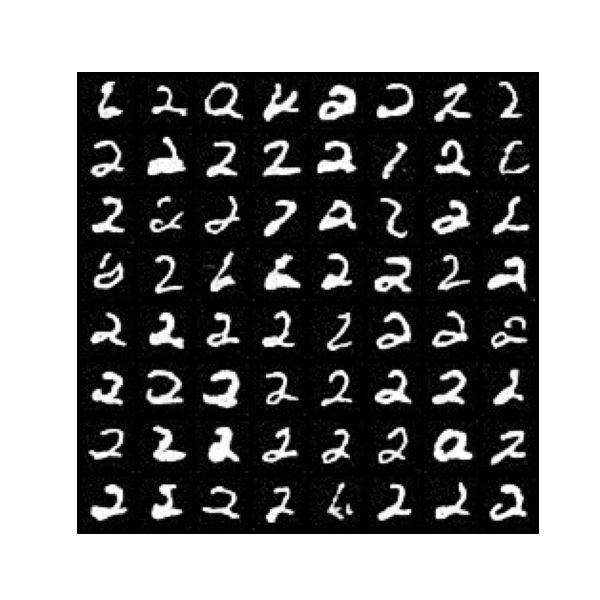
\includegraphics[width=\textwidth]{Chapters/figures/experiments/mnist/mnist_2.png}
    \end{subfigure}
    \begin{subfigure}{0.3\textwidth} \label{abb:1a}
        \centering
        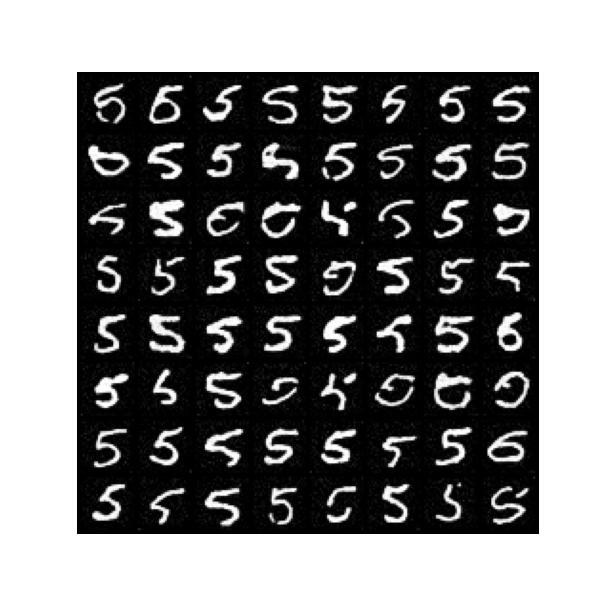
\includegraphics[width=\textwidth]{Chapters/figures/experiments/mnist/mnist_5.png}
    \end{subfigure}
    \begin{subfigure}{0.3\textwidth} \label{abb:1a}
        \centering
        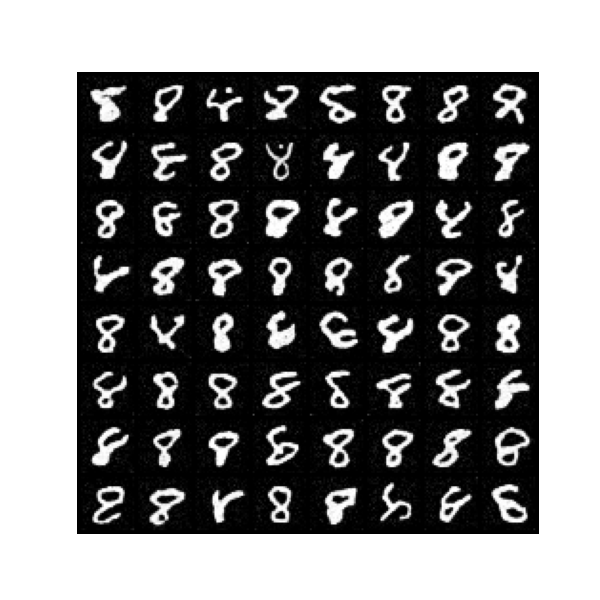
\includegraphics[width=\textwidth]{Chapters/figures/experiments/mnist/mnist_8.png}
    \end{subfigure}
    
    \caption[MNIST class-conditional results]{MNIST class-conditional results. \textit{Left:} 2, \textit{Middle:} 5, \textit{Right:} 8}
    \label{fig:my_label}
\end{figure}
%

%%%%%%%%%%%%%%%%%%%%%%%%%%%%%%%%%%%%%%%%%%%%%%%%%%%%%%%%%%%%%%%%%%%%%%%%%%%%%%%%%%%%%%%%%
\section{Semantic Synthesis Implementation} \label{sec:5.2}
As described in \hyperref[sec:4.5]{Sec.\,4.5} a semantic segmentation network is needed to learn the forward process $\log p_t(\vec{y}|\vec{x}(t))$ which can be then used to solve the $\vec{y}$-dependent reverse SDE in \hyperref[equ:4.22]{Equ.\,4.22}. Effectively this means that the semantic segmentation is learned on noisy images $\vec{x}(t)$, where the noise for timestep $t$ is governed by the forward SDE. Since for each training image $\vec{x}(0)$ there also is a segmentation map $\vec{y}$, the guess $\tilde{\vec{y}}$ of the segmentation network can be compared to the true map to then compute an error. 

\subsection{Generating noisy training images}

As mentioned above – because the forward SDE is tractable – we can easily generate as much noisy training images as we want by adding noise to the initial training images $\{\vec{x}_i(0)\}_{i=1}^N$:
%
\begin{equation} \label{equ:5.1}
    \vec{x}(t)=\vec{x}(0)+\sigma(t)\cdot\vec{z}\,.
\end{equation}
%
In \hyperref[equ:5.1]{Equ.\,5.1} $\vec{z}\sim\mathcal{N}(0, \vec{I})$ is Gaussian noise and $\sigma(t)$ is the noise scale for timestep $t$ which for the VE SDE is given by
%
\begin{equation} \label{5.2}
    \sigma(t)=\sigma_{min}\cdot\left(\frac{\sigma_{max}}{\sigma_{min}}\right)^t.
\end{equation}
%
$\sigma_{min}$ corresponds to $\sigma(t=0)$ and is always chosen as $0.01$. Since the image information is in the range $[0,1]$, a noise of $0.01$ is not visible to the human eye. $\sigma_{max}$ corresponds to $\sigma(t=T\triangleq1)$ and is chosen as the maximum pairwise distance for the dataset under investigation. During training, for each not noisy training image in a batch we then randomly choose noise scales $\sigma(t)$ with $t\in[0,1]$ and transform the not noisy training batch into a noisy training batch by using \hyperref[equ:5.1]{Equ.\,5.1}.

\subsection{Choosing a noise encoding}

With the noisy images we can now train a semantic segmentation network. Obviously a semantic segmentation network is expected to perform increasingly worse on increasingly noisy images. To give an idea of the difficulty of the task, the maximum noise scale for the Cityscapes dataset is $338$, i.e. in images with maximum noise, the noise is $338$ higher than the underlying image information! Therefore, we cannot simply train a regular segmentation network $p_\theta(\vec{x}(t))$ on noisy images, but we need to condition the network on noise $p_\theta(\vec{x}(t), \sigma(t))$, so that it can better distinguish the noise scales. There are some advanced ways to encode this noise information, including \textit{Sinusoidal Positional Embeddings} \cite{attention} or \textit{Gaussian Fourier Embeddings} \cite{fourfeat}. These encoding techniques are used in NCSN++ to encode the noise information but for the segmentation network, we work with a much simpler type of encodings.

Our idea to condition the semantic segmentation is to encode the noise information as a $4th$ channel dimension in addition to the $3$ color channels for each pixel. The size of a batch of (noisy) training image has the size $N\times C\times H\times W$. We want to expand the noise information of size $N$ to size $N\times 1\times H\times W$ and then concatenate the noise with the images to obtain a resulting batch of size $N\times (C+1)\times H\times W$. This batch is then fed into the network.

However, there are several plausible options to express the noise of an image. The first option would be to use the noise scale itself, the second option would be to use the logarithm of the noise scale and the third option would be to use the timestep which directly correlates to noise. Recalling to the noise function in \hyperref[equ:5.2]{Equ.\,5.2} we can plot these three options in \hyperref[fig:5.2]{Fig.\,5.2}.

In order to evaluate these possibilities, one needs to know the input format of the images into the network. Normally the pixel values are displayed in the range $[0, 1]$ rather than in the range $[0, 255]$. But since there is noise added to the initial images the pixel ranges can be everywhere from $[0,\sigma_{min}]$ and $[0, \sigma_{max}]$, depending on the current noise scale. When we tried to learn a segmentation network from images in various pixel ranges we got very bad results. Therefore, we transform any perturbed image $\vec{x}(t)$ into the range $[0, 1]$ by using the following formula:
%
\begin{equation}
    \vec{x}_{[0,1]}(t)=\frac{\vec{x}(t)-\min(\vec{x}(t))}{\max(\vec{x}(t))-\min(\vec{x}(t))}.
\end{equation}
%

It is plausible that the noise encodings should be in a related order of magnitude than the image information. Therefore, we do not use noise scales as encodings because they are up to two magnitudes larger. Training one segmentation network conditioned on the logarithm of the noise scale $\log \sigma(t)$ and another conditioned on timesteps $t\in[0,1]$ revealed no significant differences. After $100$ epochs on the cityscapes dataset we got a peak IoU of $\sim0.212$ for noise encodings and a peak IoU of $\sim0.213$ for timestep encodings. Since NCSN++ is conditioned on the logarithm of the noise scale, we also choose this encoding to condition our semantic segmentation network $p_\theta(\vec{x}(t), \log \sigma(t))$.

\subsection{Choosing a Semantic Segmentation Network}

There exists a wide variety of semantic segmentation networks that we could use. The problem with state-of-the-art segmentation networks is, that they often use pretrained classification networks in their architecture which makes them hard to condition on noise, because these pretrained networks are obviously not trained on noisy images. 

Therefore, we first tried to use simpler models such as U-Net (\hyperref[sec:3.1.2]{Sec.\,3.1.2}) which are easy to implement and easy to condition on noise. The results we got were not really promising but it turned out that they actually were good enough to use them for semantic image synthesis. Concrete analyses of the trained segmentation networks in terms of pixel accuracy and IoU is presented in the dedicated experiment sections \hyperref[sec:5.4]{Sec.\,5.4}, \hyperref[sec:5.5]{Sec.\,5.5} and \hyperref[sec:5.6]{Sec.\,5.6}.

We also tried to condition more complicated networks such as FCDenseNet \cite{densenet}, which significantly outperforms U-Net on non-noisy images, but we could only achieve a peak IoU of $\sim0.146$ on noisy images, so we finally decided to use U-Net as semantic segmentation network for further experiments.

\subsection{Choosing an error function}

To compare the estimated semantic map $\tilde{\vec{y}}$ with the ground truth semantic map $\vec{y}$, we need to specify an error function. For U-Net the cross-entropy loss function is a good choice. Cross-entropy calculates the loss for an output given as probability value between $0$ and $1$ which is exactly what we (pixel-wise) have for a semantic segmentation network. The cross entropy operates on the logarithm of the output probability $\log p$. If the true label of a pixel is $1$ the loss is relatively low for probabilities $>0.2$ and grows rapidly for lower losses. For multiclass classification as for semantic segmentation the cross-entropy loss can be written as
%
\begin{equation}
    \Delta_{xy}=-\sum_{c=1}^C 
    \begin{cases}
        0, &\text{for } c\neq c_t\\
        \log p(c_t)_{xy}, &\text{otherwise}
    \end{cases}
\end{equation}
%
where $C$ is the total number of labels, $x$ and $y$ are the pixel-wise positions in the segmentation map, $c_t$ is the true label for position $xy$ and $p(c_t)_{xy}$ is the probability the network outputs for the pixel at position $xy$ having label $c_t$.
%
\subsection{Choosing a scale factor function} \label{sec:5.2.5}
As already touched upon in the previous section \hyperref[sec:5.1]{Sec.\,5.1} a scale factor for the gradients of the semantic segmentation network is necessary to obtain good sampling results. When using a static scale factor, we observe that the pixel values often go into saturation, i.e. converging to $1$, which leads to overexposed samples (see e.g. sample for $T=0$ in \hyperref[fig:5.3]{Fig.\,5.3}). 

We are therefore interested in finding the time interval $T\subset[0,1]$ in which the gradients of the semantic segmentation network are the most needed, i.e. in which time interval important structural image information is formed and consolidated. With this information we hope to reduce the saturation effect on the final sample, because the semantic segmentation network is influencing the sample for a lower amount of time. We propose that for low noise ($t$ near $0$) the image structure is already consolidated and the semantic segmentation network only plays a minor role for generation. We further propose that for high noise ($t$ near $1$) the gradients of the segmentation network in theory would be beneficial for generation, but only if the network is capable to operate on high noise scales which we could not achieve up to maximum noise.

Therefore, as a scaling function we propose a function that is $0$ in regions where the network performs badly and $1$, in regions where the networks performs reasonable, followed by a linear decrease to $0$ for regions where we suggest that the image structure has already consolidated. To find out these regions we perform two experiments. In the first experiment we set the scale factor to $1$ for $t>t_{stop}$ and to $0$ for $t\leq t_{stop}$, where $t_{stop}$ is subsequently reduced from $1$ to $0$ for each sample. In the second experiment we introduce $t_{start}$ for which for $t<t_{start}$ the scale factor is $1$ and for $t\geq t_{start}$ the scale factor is $0$. The results – exemplary for one semantic map – can be seen in \hyperref[fig:5.4]{Fig.\,5.4} resp. \hyperref[fig:5.5]{Fig.\,5.5}.

%
\begin{figure} \label{fig:5.2}
    \centering
    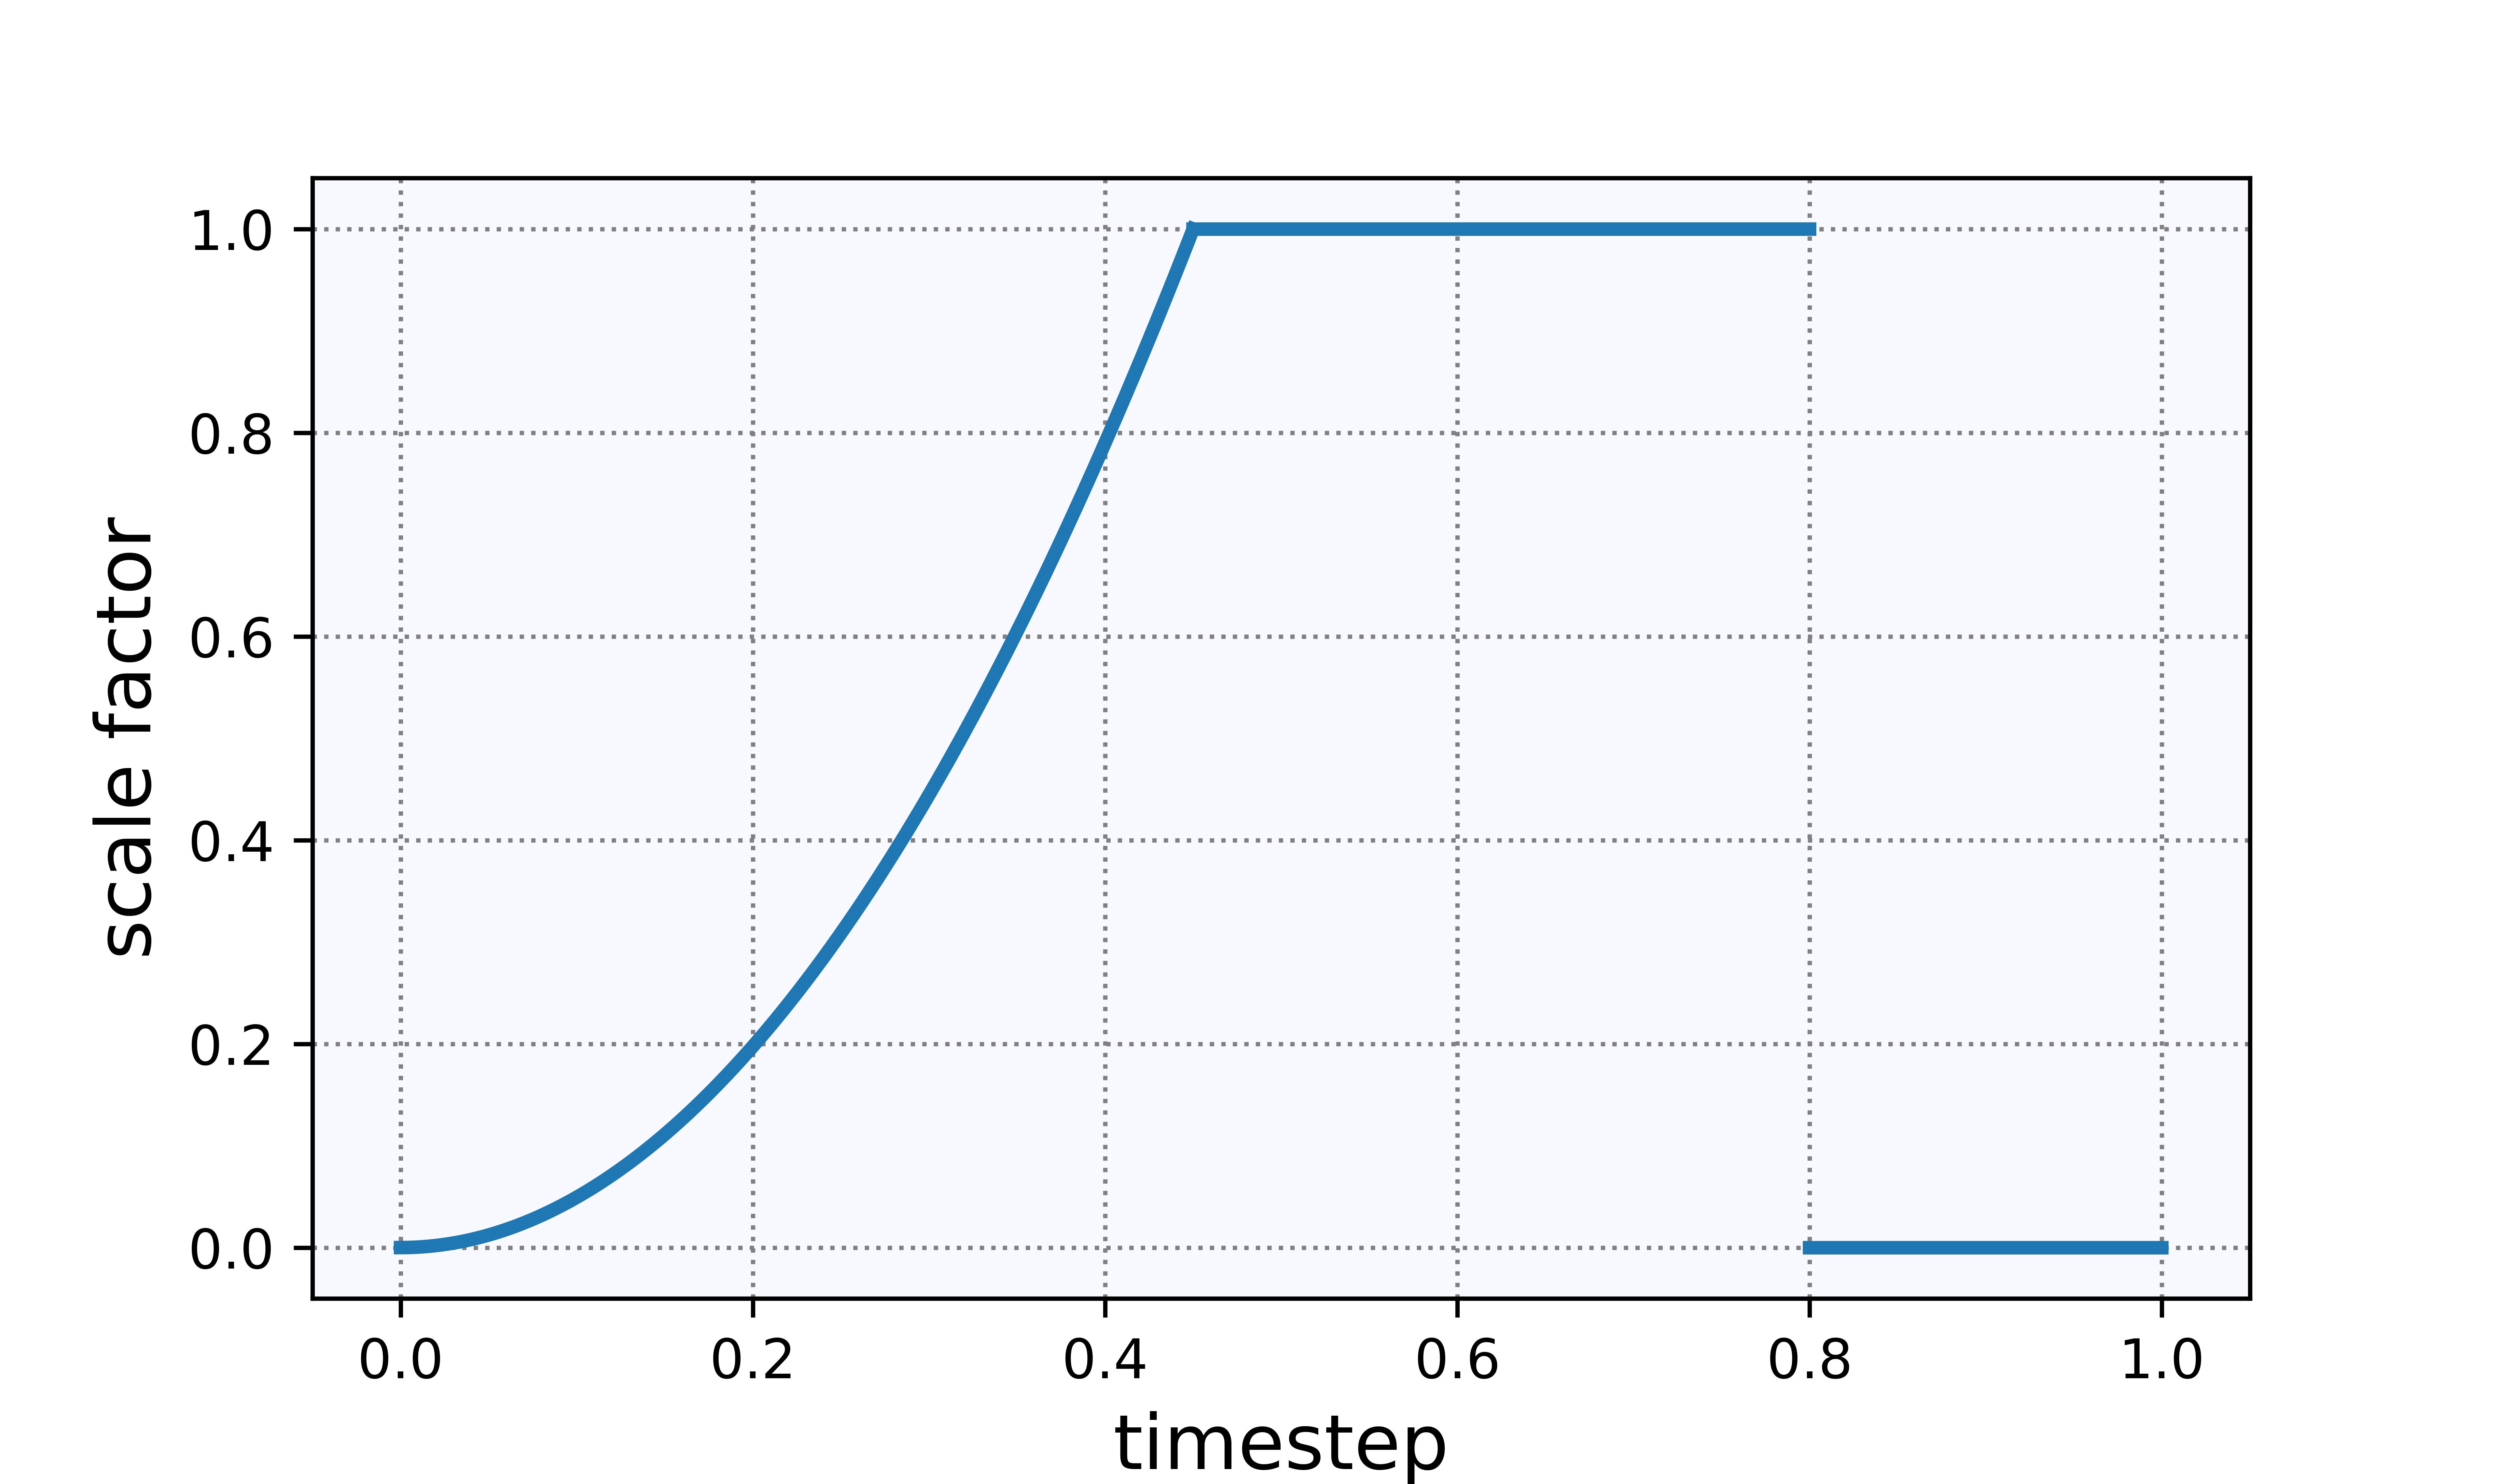
\includegraphics[width=.65\textwidth]{Chapters/figures/experiments/scale/scale_function.jpg}
    \caption{The proposed scale factor function}
\end{figure}
%
We come to the qualitative result that in order to get samples that match the semantic map the semantic segmentation network has to be started at $t>65$ and can be stopped/decreased at $t<0.45$.  Based on the findings for these experiments, supplemented by the accuracy and mIoU curves in TODO, we generously conclude that for $t>0.8$ the segmentation network performs to badly to be helpful for generation and that for $t<0.45$ the structures in the image have already consolidated. We therefore propose the following scale function:
%
\begin{equation} \label{equ:5.5}
    s(t)=\begin{cases}
        0, &\text{for }t>0.8\\
        s_0, &\text{for }t\leq0.8 \land t>0.45\\
        \frac{s_0}{0.45^2}t^2, &\text{for }t\leq0.45
    \end{cases},
\end{equation}
%
where $s_0$ is the maximum scale factor for a given dataset, which is determined experimentally. As function in the region $0\leq t\leq0.45$ any kind of function that decreases sufficiently fast could be used. The final gradients for sampling are therefore calculated via
%
\begin{equation}
    \nabla_{\vec{x}}\log p_t(\vec{x})+s(t)\cdot\nabla_{\vec{x}}\log p_t(\vec{y}|\vec{x}).
\end{equation}

\begin{figure} \label{fig:5.4}
    \tiny
    \centering
    \setlength\tabcolsep{-2pt}
    \begin{tabular}{cccc}
        Semantic map & Original image & T=0.8 & T=0.7 \\
        \includegraphics[width=0.25\textwidth]{Chapters/figures/experiments/seg_stop/0_1.0_seg_mask.png} &  \includegraphics[width=0.25\textwidth]{Chapters/figures/experiments/seg_stop/0_1.0_original.png} & 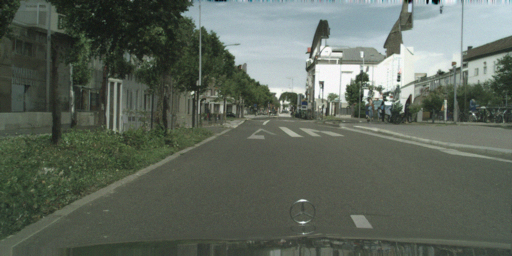
\includegraphics[width=0.25\textwidth]{Chapters/figures/experiments/seg_stop/0_0.8_cond_sample.png} & 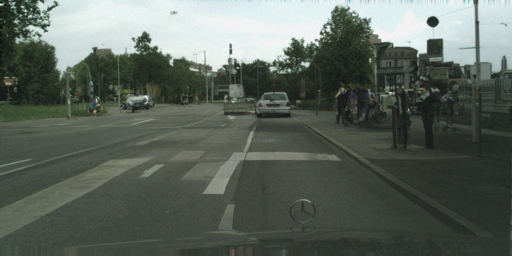
\includegraphics[width=0.25\textwidth]{Chapters/figures/experiments/seg_stop/0_0.7_cond_sample.png} \\
        T=0.65 & T=0.6 & T=0.55 & T=0.5\\
        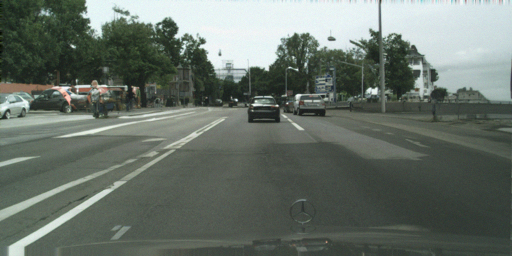
\includegraphics[width=0.25\textwidth]{Chapters/figures/experiments/seg_stop/0_0.6499999999999999_cond_sample.png} & 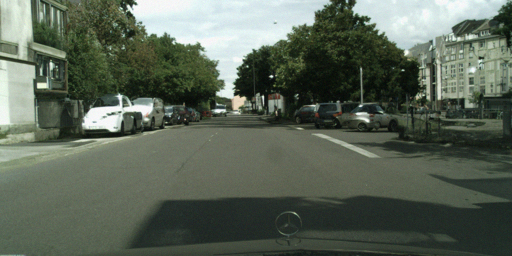
\includegraphics[width=0.25\textwidth]{Chapters/figures/experiments/seg_stop/0_0.6_cond_sample.png} & 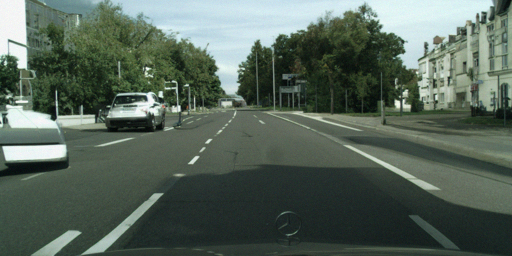
\includegraphics[width=0.25\textwidth]{Chapters/figures/experiments/seg_stop/0_0.55_cond_sample.png} & 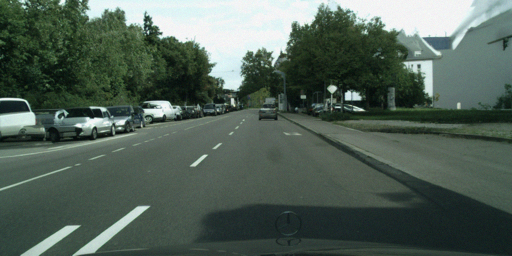
\includegraphics[width=0.25\textwidth]{Chapters/figures/experiments/seg_stop/0_0.5_cond_sample.png}\\
        T=0.45 & T=0.4 & T=0.2 & T=0\\
         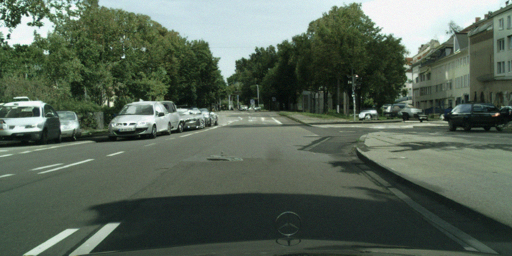
\includegraphics[width=0.25\textwidth]{Chapters/figures/experiments/seg_stop/0_0.44999999999999996_cond_sample.png} & 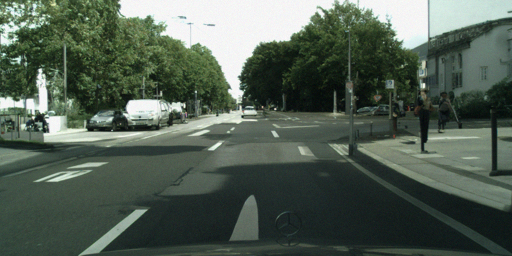
\includegraphics[width=0.25\textwidth]{Chapters/figures/experiments/seg_stop/0_0.3999999999999999_cond_sample.png} & 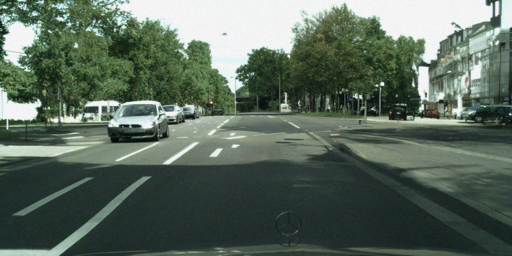
\includegraphics[width=0.25\textwidth]{Chapters/figures/experiments/seg_stop/0_0.19999999999999996_cond_sample.png}& 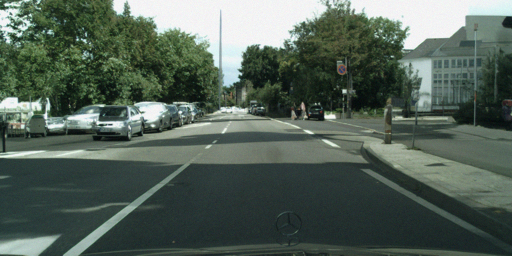
\includegraphics[width=0.25\textwidth]{Chapters/figures/experiments/seg_stop/0_0.0_cond_sample.png} 
    \end{tabular}
    \caption[Switching off the semantic segmentation network at different timesteps]{Switching off the semantic segmentation network at different timesteps $T\in[0,1]$}
\end{figure}

\begin{figure} \label{fig:5.5}
    \tiny
    \centering
    \setlength\tabcolsep{-2pt}
    \begin{tabular}{cccc}
        Semantic map & Original image & T=0.2 & T=0.4  \\
        \includegraphics[width=0.25\textwidth]{Chapters/figures/experiments/seg_start/0_1.0_seg_mask.png} & 
        \includegraphics[width=0.25\textwidth]{Chapters/figures/experiments/seg_start/0_1.0_original.png} & 
        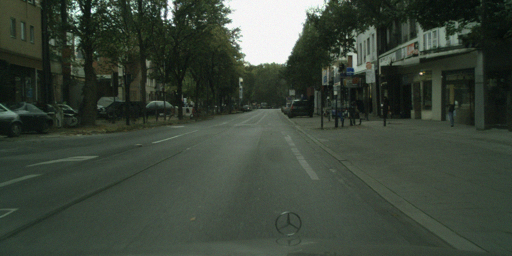
\includegraphics[width=0.25\textwidth]{Chapters/figures/experiments/seg_start/0_0.19999999999999996_cond_sample.png} & 
        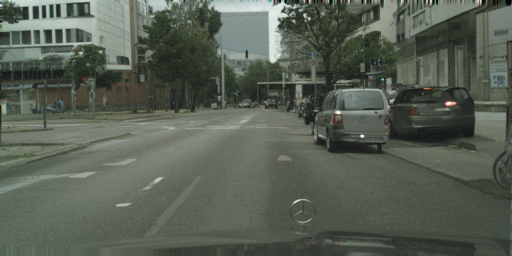
\includegraphics[width=0.25\textwidth]{Chapters/figures/experiments/seg_start/0_0.3999999999999999_cond_sample.png} \\
        T=0.5 & T=0.6 & T=0.65 & T=0.7  \\
        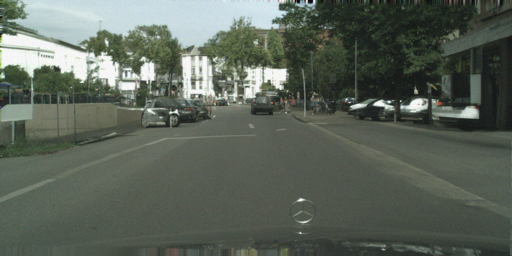
\includegraphics[width=0.25\textwidth]{Chapters/figures/experiments/seg_start/0_0.5_cond_sample.png} & 
        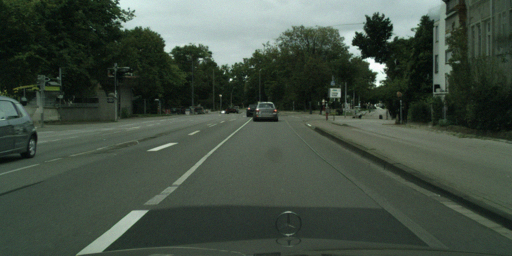
\includegraphics[width=0.25\textwidth]{Chapters/figures/experiments/seg_start/0_0.6_cond_sample.png} & 
        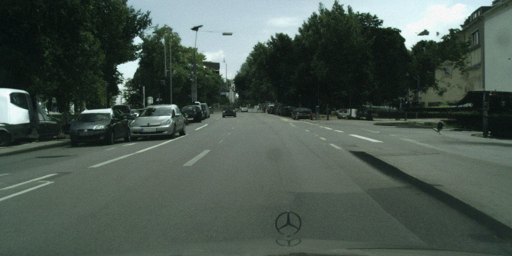
\includegraphics[width=0.25\textwidth]{Chapters/figures/experiments/seg_start/0_0.6499999999999999_cond_sample.png} &
        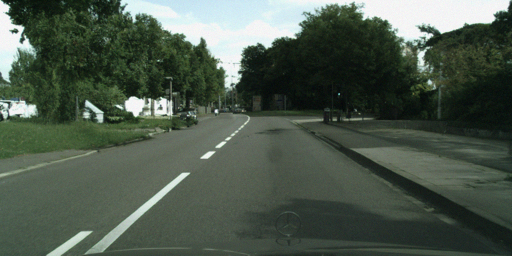
\includegraphics[width=0.25\textwidth]{Chapters/figures/experiments/seg_start/0_0.7_cond_sample.png}  \\
        T=0.75 & T=0.8 & T=0.9 & T=1  \\
        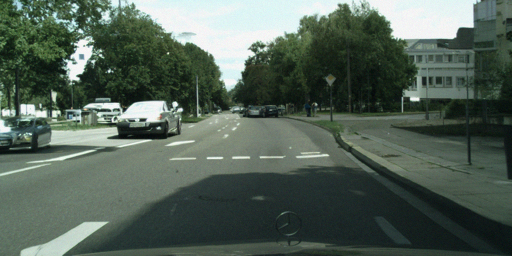
\includegraphics[width=0.25\textwidth]{Chapters/figures/experiments/seg_start/0_0.75_cond_sample.png} & 
        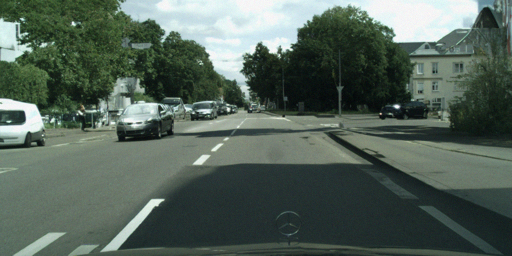
\includegraphics[width=0.25\textwidth]{Chapters/figures/experiments/seg_start/0_0.8_cond_sample.png} & 
        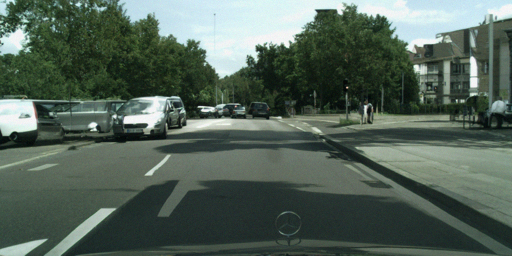
\includegraphics[width=0.25\textwidth]{Chapters/figures/experiments/seg_start/0_0.9_cond_sample.png} & 
        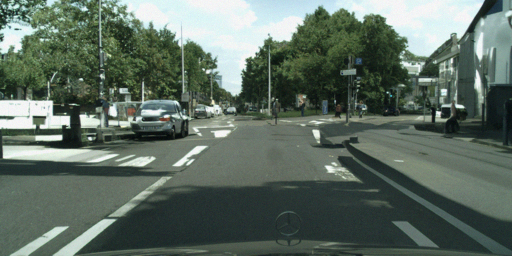
\includegraphics[width=0.25\textwidth]{Chapters/figures/experiments/seg_start/0_1.0_cond_sample.png}
    \end{tabular}
    \caption[Switching on the semantic segmentation network at different timesteps]{Switching on the semantic segmentation network at different timesteps $T\in[0,1]$}
\end{figure}
%%%%%%%%%%%%%%%%%%%%%%%%%%%%%%%%%%%%%%%%%%%%%%%%%%%%%%%%%%%%%%%%%%%%%%%%%%%%%%%%%%%%%%%%%%
\section[Improvements and Adaptations]{Improvements and Adaptations%
    \sectionmark{Improvements}} \label{sec:5.3}
\sectionmark{Improvements}
As initial experiments before testing semantic image synthesis on a large scale, we test the impact of two improvements/adaptations we made to the original score model architecture \cite{score_3}.
\subsection{Mixed precision learning} \label{sec:5.3.1}
vRAM usage and training speed are key aspects in training deep neural network. Complex models might consist of several million up to billion parameters to optimize. This requires an immense amount of computing power but at least equally important, vRAM. vRAM – video random access memory – is the memory that a GPU has available during operation. Modern high end consumer graphic cards typically have around $10GB$ of vRAM. The crux of the matter is that reaching more than $10GB$ when training a moderately complex model is really easy and when training such complex models as NCSNs, the vRAM demand can increase beyond $100GB$, making training deep neural networks a very cost intensive business. Also, when training complex models one can expect to need one week or more of training time, making testing and finetuning of models very exhausting.

To mitigate these problems the concept of \textit{Mixed Precision Learning} \cite{mixed_prec} was developed, decreasing both vRAM usage and training time with simultaneous retention of training quality, i.e. training loss. Normally each parameter of a network is stored as a float with $32bits$ of precision. Considering a network with $\sim250M$ parameters this would be equivalent to $\sim1GB$. What sounds not so much at first quickly becomes unmanageable when thinking of the series of matrix arithmetic's the parameters undergo and each calculation storing extra data such as gradients. 

The idea of mixed precision learning is to use floats with a $16bit$ precision wherever possible. In order to not lose model accuracy two concepts are applied. First, there is always a $32bit$ master copy of the model weights. For the forward pass this master copy is converted to $16bit$, where the complex gradient calculations happen. In the backward pass these $16bit$ gradients are converted back to $32bit$ where they are then used by the optimizer to update the master weights. But this improvement during gradient calculation comes with the flaw of losing some gradients as every number $<2^{-24}$ is equal to $0$ for $16bit$ precision but in most models there is at least some relevant gradient information in the range $[2^{-27},2^{-24})$. To mitigate this effect the concept of loss scaling was proposed. Loss scaling multiplies the $32bit$ loss after the forward pass by a scale factor to move them in the $16bit$ range in which the gradients are then computed in the backward pass. Thereafter the scaled $16bit$ gradients are converted to scaled $32bit$ gradients and then divided by the same scale factor as before. Finally, these scaled gradients are used by the optimizer to update the master weights. The full concept can be seen in \hyperref[fig:3.2]{Fig. 3.2}.
%
\begin{figure}[] \label{fig:3.2}
    \centering
    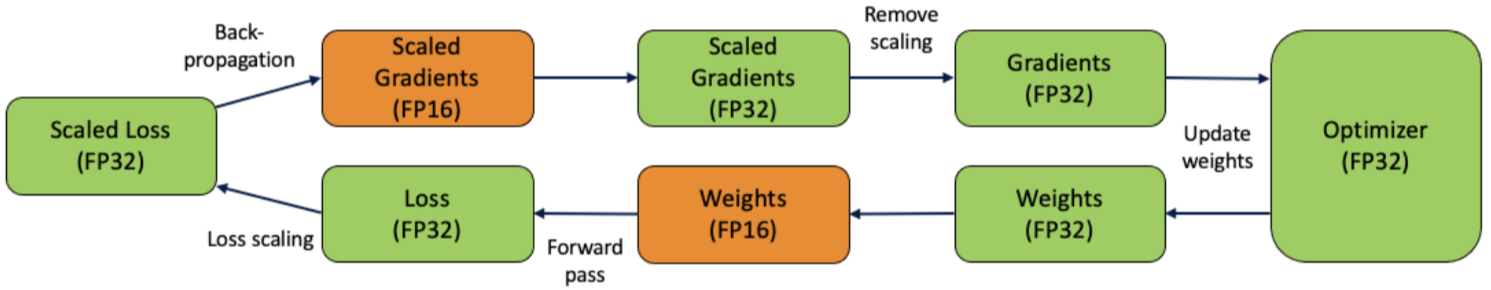
\includegraphics[width=.9\textwidth]{Chapters/figures/mixed_prec.PNG}
    \caption{Concept of Mixed Precision}
\end{figure}
%

As the mixed precision technique was not used in the original SGM paper \cite{score_3} it was now implemented using the off-the-shelf PyTorch tools for mixed precision to check how much this technique improves vRAM usage and training time for the NCSN. To do so we trained the NCSN++ on the Cityscapes dataset on two different GPUs with the same model settings. For each GPU $2\times100$ epochs were passed, once with mixed precision on and once with mixed precision off. The first GPU was a \textit{Nvidia GeForce RTX 2080 Ti} with $11GB$ of vRAM and the second GPU was a \textit{Nvidia A100} with $40GB$ of vRAM. For both GPUs we used the maximum possible batch size for non-mixed precision training which is $1$ for the RTX 2080 Ti and $5$ for the A100. The effects of mixed precision training on vRAM usage and training time can be seen in \hyperref[tab:3.1]{Tab. 3.1} resp. \hyperref[tab:3.1]{Tab. 3.2}. For the vRAM usage the total vRAM needed is shown and for the training time the average training time for one epoch is shown.
%
\begin{table}[] \label{tab:3.1}
        \centering
    \begin{tabular}{c|c|c}
        \toprule
        GPU type        & Mixed precision \textbf{Off}    & Mixed precision \textbf{On} \\
        \midrule
        RTX 2080 Ti     &  7791MB               & 7367MB\\
        A100            &  39039MB              & 29481MB\\
        \bottomrule
    \end{tabular}
    \caption{vRAM usage w/ and w/o mixed precision}
\end{table}
\begin{table}[b] \label{tab:3.2}
        \centering
    \begin{tabular}{c|c|c}
        \toprule
        GPU type        & Mixed precision \textbf{Off}    & Mixed precision \textbf{On} \\
        \midrule
        RTX 2080 Ti     &  1494s                & 1206s    \\
        A100            &  965s                 & 987s\\
        \bottomrule
    \end{tabular}
    \caption{Training time per epoch w/ and w/o mixed precision}
\end{table}

For the A100 serious improvements on vRAM usage can be observed. For the RTX 2080 Ti there are only little improvements for vRAM usage but good improvements on training time. In general, mixed precision is expected to perform way better on the new Ampere GPU
architecture (A100) than on the older Turing GPU architecture (RTX 2080 Ti). To ensure that the training quality does not suffer from the use of mixed precision the loss curves for all test setups are compared in \hyperref[fig:3.3]{Fig. 3.3}. The higher fluctuations for the RTX 2080 Ti are due to the fact that the batch size is smaller, therefore leading to major loss differences in a batch-to-batch comparison. In general, it can be seen that mixed precision has no notable effect on training loss. Also, a qualitative comparison of generated samples shows no difference perceptible by a human. We therefore conclude that – at least for non-FID records breaking attempts – mixed precision should be used and we do so for all upcoming experiments. It should be noted, however, that in a few cases, unstable behavior occurred during mixed-precision learning, resulting in $nan$ values at training loss. In these cases, the run had to be discarded.
%
\begin{figure} \label{fig:3.3}
    \centering
    \begin{subfigure}[b]{0.49\textwidth}
        \centering
         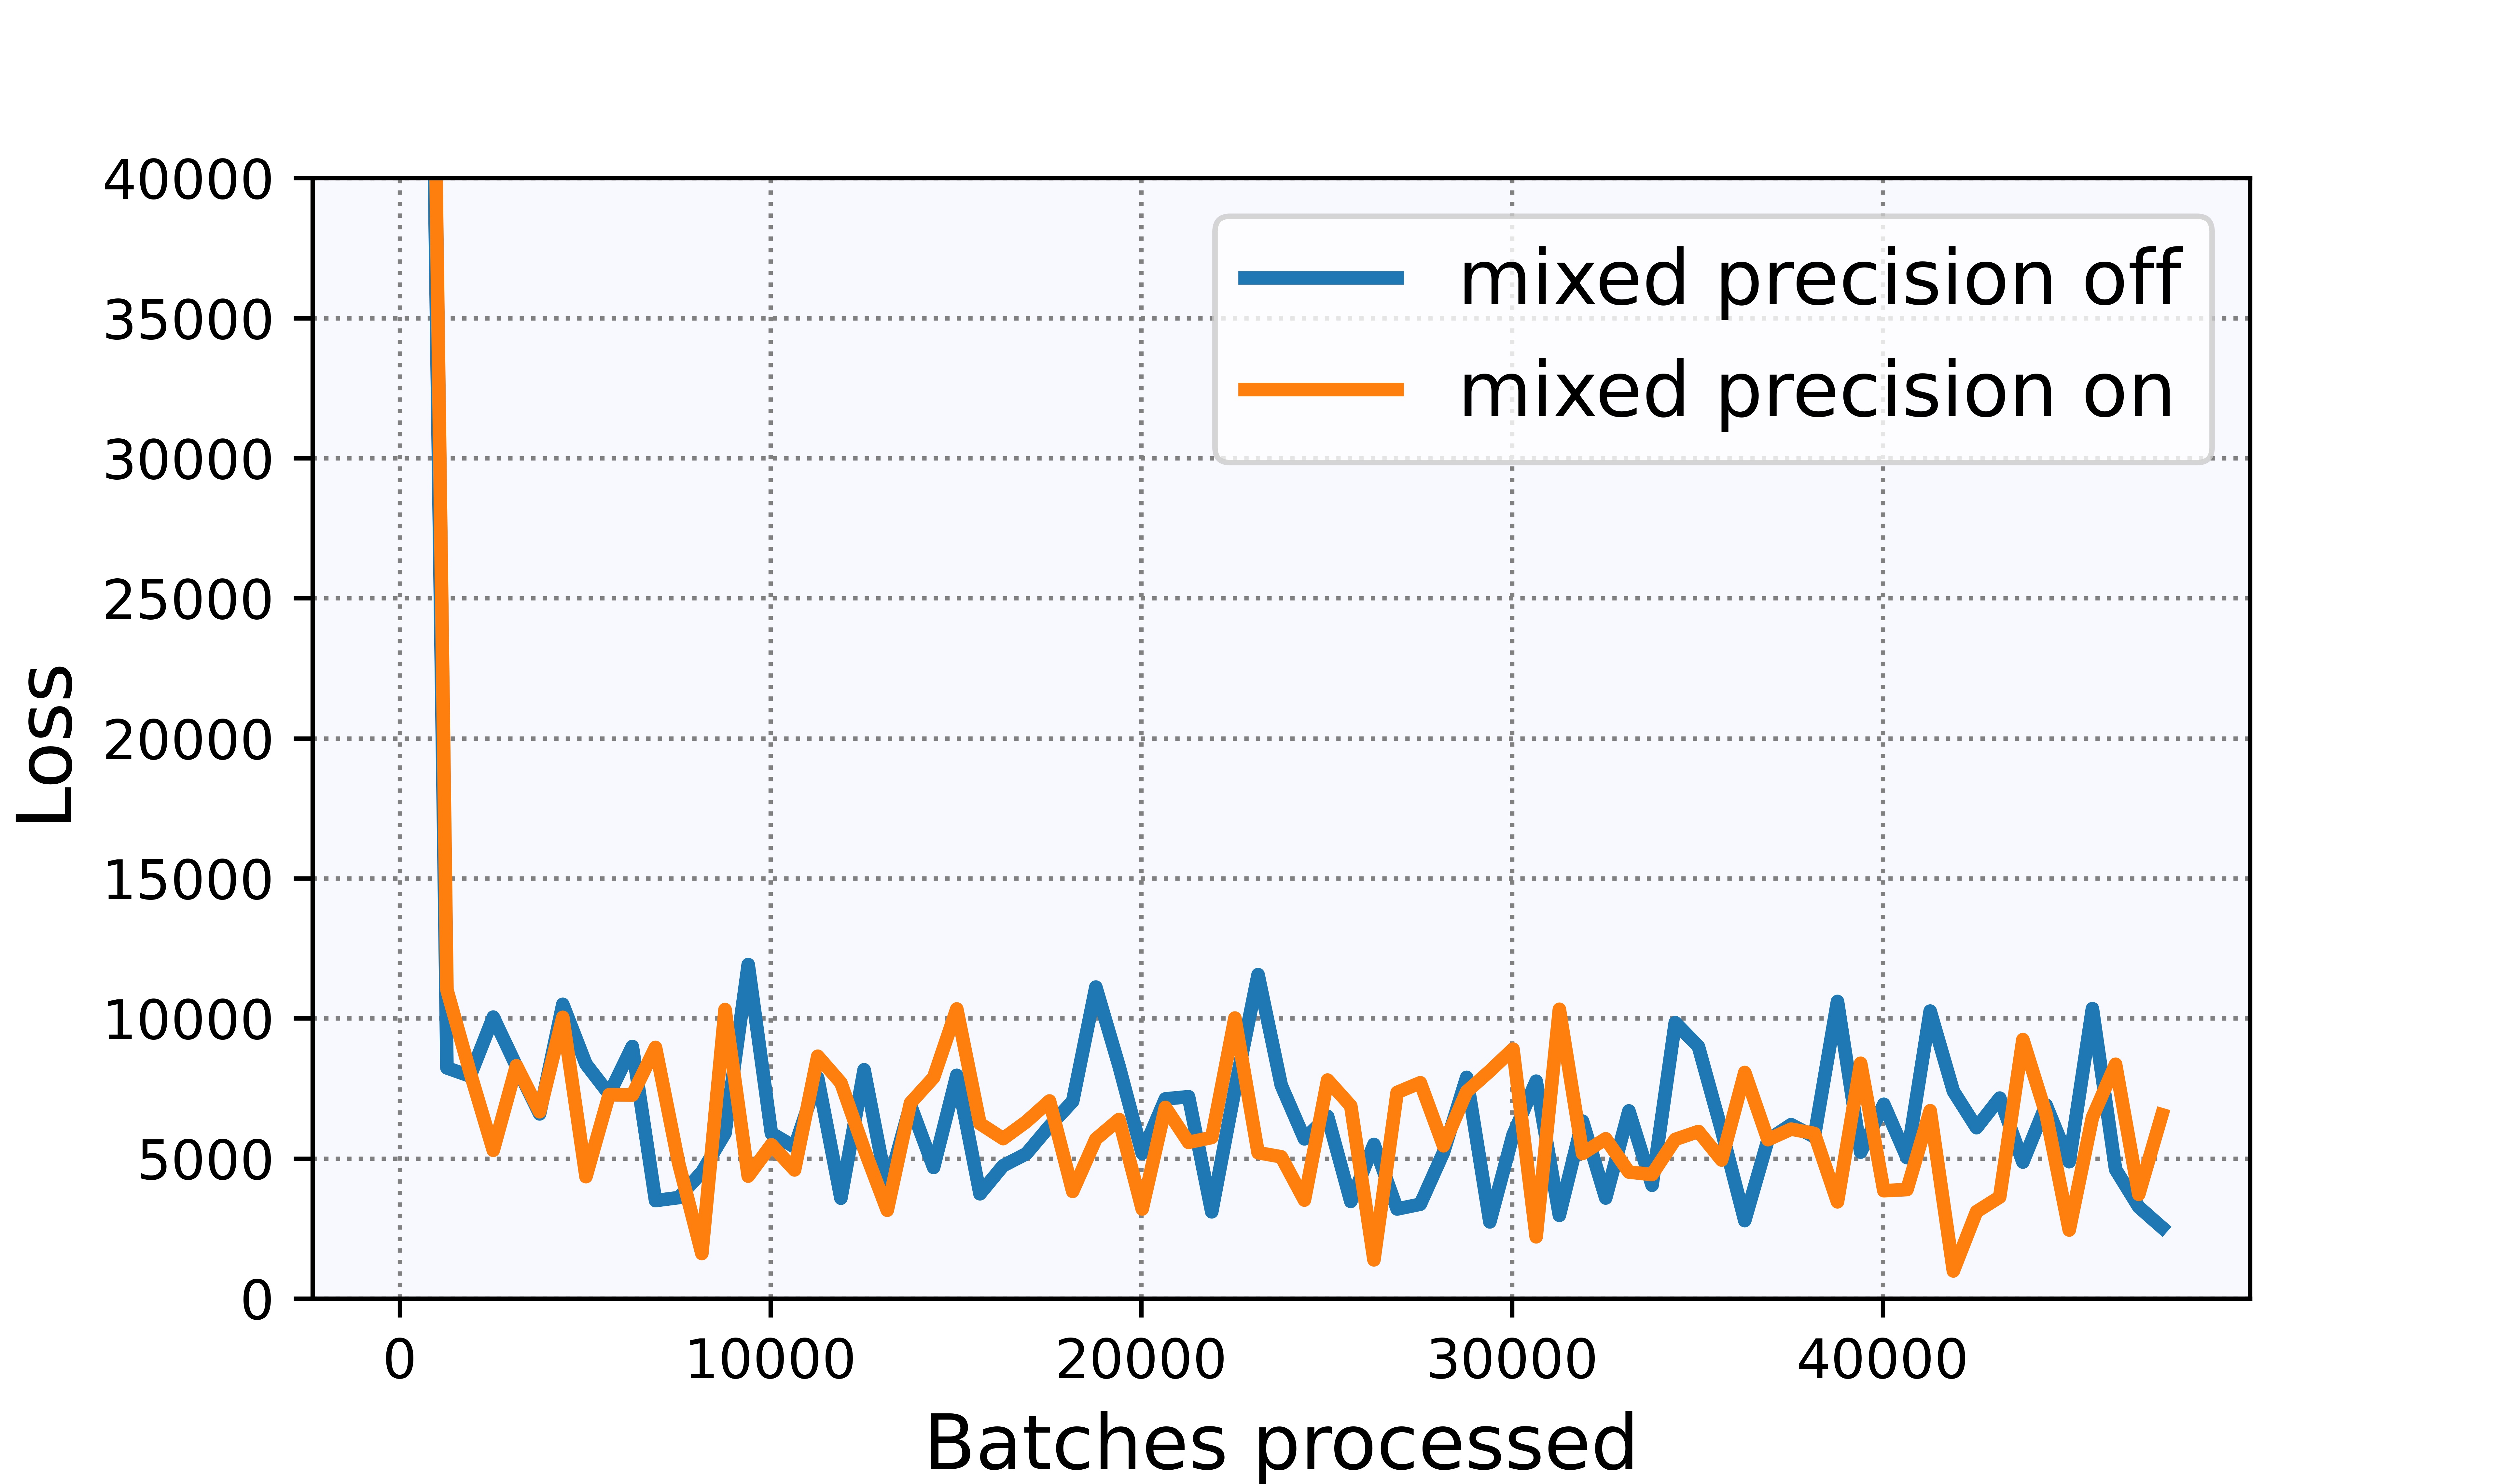
\includegraphics[width=\textwidth]{Chapters/figures/mixed_prec_rtx2080_loss.jpg}
         \caption{Loss curve RTX 2080 Ti}
    \end{subfigure}
    \begin{subfigure}[b]{0.49\textwidth}
        \centering
         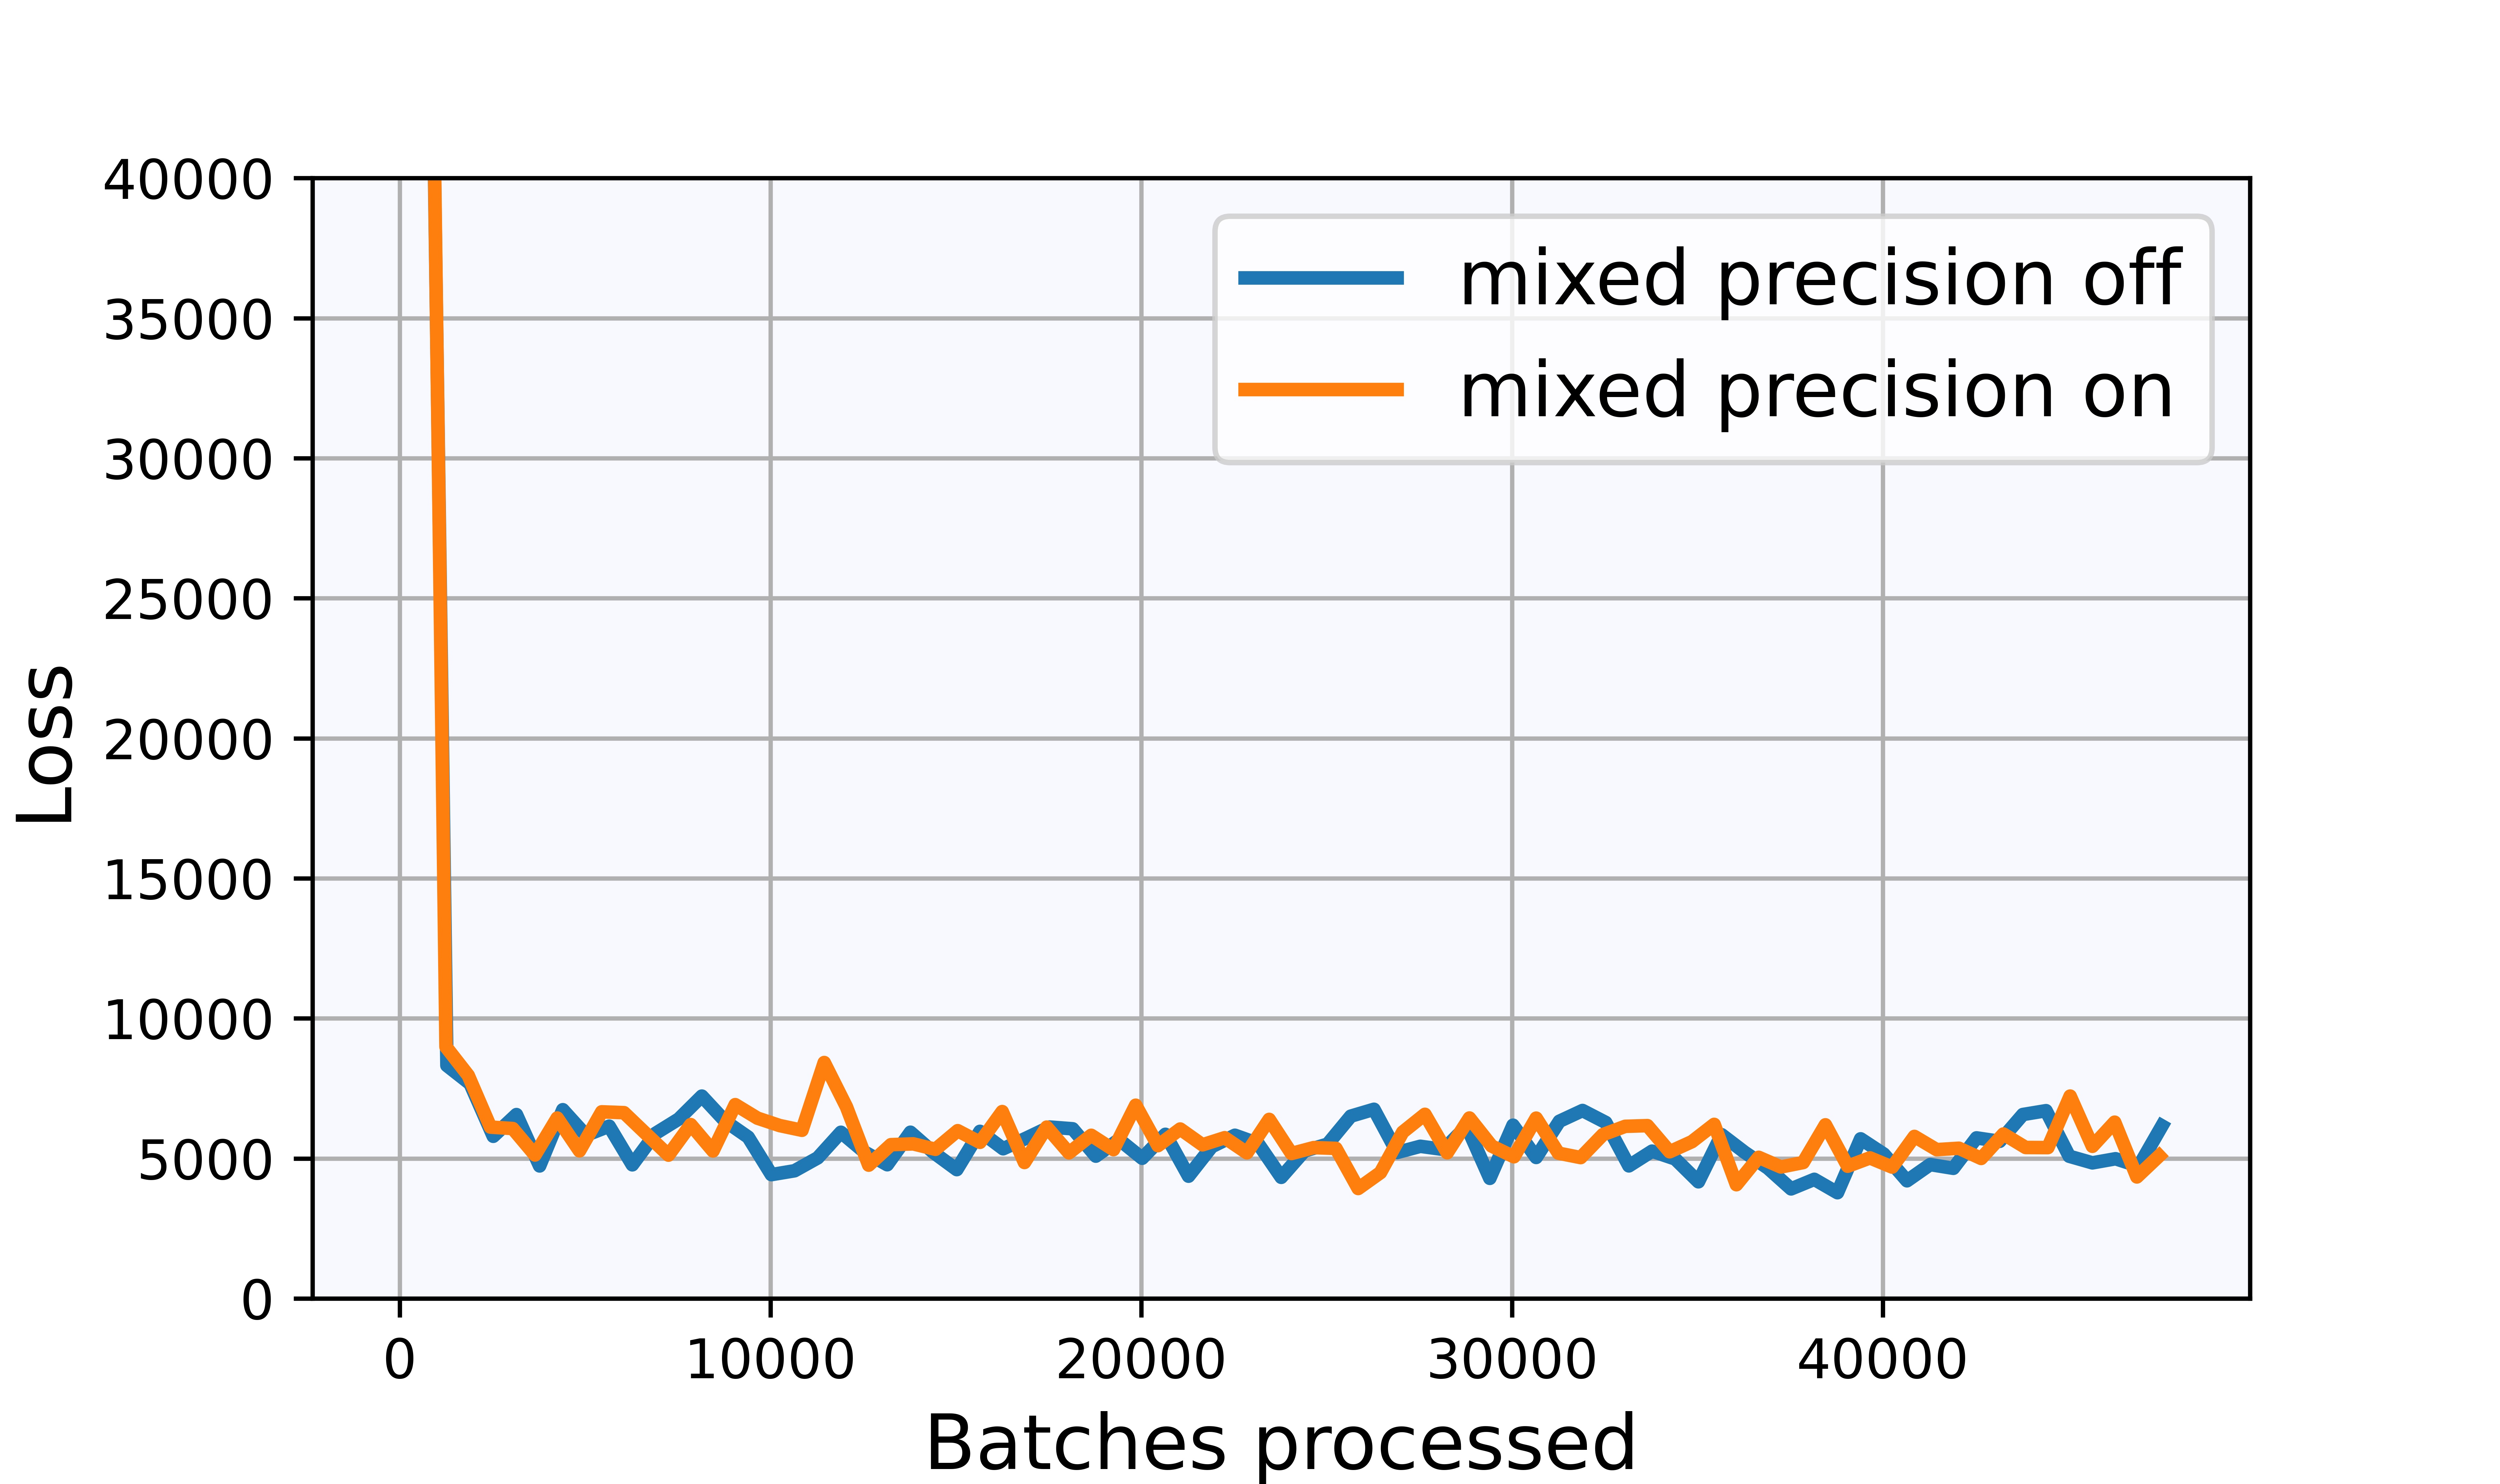
\includegraphics[width=\textwidth]{Chapters/figures/mixed_prec_a100_loss.jpg}
         \caption{Loss curve A100}
    \end{subfigure}
    \caption{Comparing loss curves for mixed precision \textbf{on} an \textbf{off} for both GPUs}
\end{figure}
%
\subsection{Training on arbitrary image sizes} %0.5-1
When training a generative model, the image size the model gets as input for learning can have a large effect on what the model learns. Here not the total image size of the images is meant but the image size the model gets as input. As an example, the cityscapes dataset (downscaled) consists of $256\times512$ pixel images. To reduce vRAM during training, the images from the dataset often are randomly cropped to another resolution, here $256\times256$ pixels. For some datasets this has only little negative effects on the model accuracy, e.g. for landscapes where the relative position of objects to each other only plays a minor role. But for datasets as the cityscapes dataset it is quite important for realistic results that the model learns the logic of images showing street scenes, i.e. learning that the street is in the middle, that there are parking cars on the left and right side of the image and so on. Training on too small crops can hinder the model to learn such logic.

As the version of NCSN \cite{score_3} does not support training on/sampling of non-square images, the model was adapted to do so. Actually, the model already was able to process non-square images natively but there was a small bug that we fixed to make non-square training/sampling possible. To show the importance of this bugfix we investigate the influence of the above described effect on NCSN. For this purpose, we trained two identical NCSN, one on $256\times256$ pixels crops and one on the $256\times512$ pixels original images. Some example results can be seen in \hyperref[fig:]{Fig.\,TODO}. It is clearly visible that the full image model outperforms the cropped image model when the focus of evaluation is on street scene logic. It must be mentioned that for semantic image synthesis – the task for our experiments – this logic information actually is given by the semantic map which initially gives rise to the idea of training on crops at all. Nevertheless, we suspect that a model knowing the logic without a semantic map also performs somewhat better than if it did not. For that reason, models for further experiments on the cityscapes dataset were always trained with the full size images. For larger images such as landscape images from Flickr which reach resolutions up to $2048\times1024$ pixels this strategy is computationally not feasible and we chose a crop size of $512\times512$ pixels.
\begin{figure}[] \label{tab:5.3}
    \centering
    \setlength\tabcolsep{-2pt}
    \begin{tabular}{ccc}
        & Training size $256\times256$ & \\
        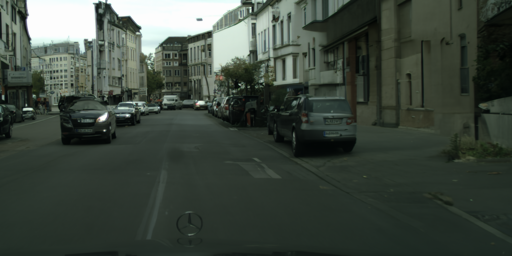
\includegraphics[width=0.33\textwidth]{Chapters/figures/experiments/crop/1_sample.png} &
        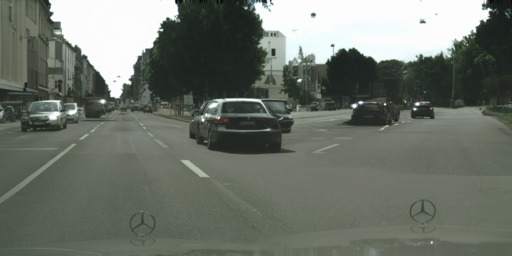
\includegraphics[width=0.33\textwidth]{Chapters/figures/experiments/crop/5_sample.png} &
        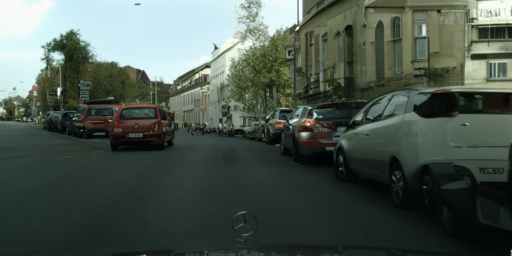
\includegraphics[width=0.33\textwidth]{Chapters/figures/experiments/crop/8_sample.png}\\
        & Training size $512\times256$ & \\ 
        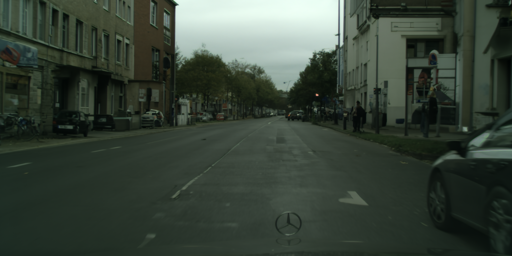
\includegraphics[width=0.33\textwidth]{Chapters/figures/experiments/crop/0_uncond_sample.png} &
        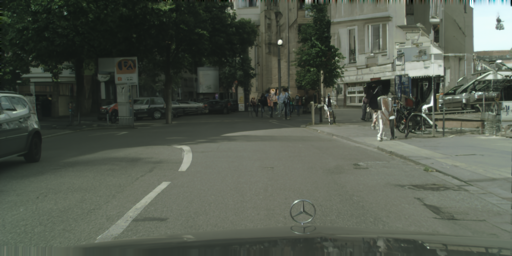
\includegraphics[width=0.33\textwidth]{Chapters/figures/experiments/crop/3_uncond_sample.png} &
        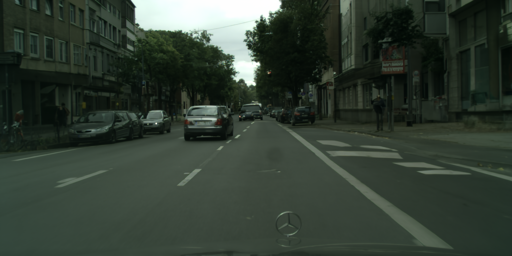
\includegraphics[width=0.33\textwidth]{Chapters/figures/experiments/crop/7_uncond_sample.png}
    \end{tabular}
    \caption[Unconditional samples of NCSN trained on cropped images and full size images]{Unconditional samples of NCSN trained on cropped images (\textit{top}) and full size images (\textit{bottom})}
\end{figure}

%%%%%%%%%%%%%%%%%%%%%%%%%%%%%%%%%%%%%%%%%%%%%%%%%%%%%%%%%%%%%%%%%%%%%%%%%%%%%%%%%%%%%%%%%%%%%%%%%

\section[A competitive experiment on the Cityscapes dataset]{A competitive experiment on the Cityscapes dataset%
    \sectionmark{Cityscapes}} \label{sec:5.4}
\sectionmark{Cityscapes}
%
As a first experiment we want to test semantic image synthesis with SGMs on the Cityscapes dataset \cite{cityscapes} (\hyperref[sec:5.4.1]{Sec.\,5.4.1}). Because of the similar image scenery in every picture and the small number of classes the Cityscapes dataset is a relatively easy and therefore popular dataset for tasks as semantic segmentation and semantic image synthesis. For computational reasons we will work on downsampled images of size $512\times256$ pixels but later experiments on landscape images (\hyperref[sec:5.5]{Sec.\,5.5}) are also tasked to generate higher resolution images. We will investigate the influence of various model and sampling parameters on sampling quality in \hyperref[sec:5.4.3]{Sec.\,5.4.3}. Thereafter we will compare our resulting samples with state-of-the-art semantic image synthesis models in \hyperref[sec:5.4.4]{Sec.\,5.4.4} using the evaluation metrics described in \hyperref[sec:5.4.2]{Sec.\,5.4.2} and a human perceptual study.

\subsection{The Cityscapes dataset}
The Cityscapes dataset \cite{cityscapes} is a dataset containing pictures of street scenes shot in various German cities in daylight and good/medium weather conditions. It contains $5000$ $2048\times1024$ $8bit$ color images with a fine annotated label map for each image. Moreover, it contains $20{,}000$ images with coarse annotated label maps which were not used for the experiments. $500$ of the $5000$ images/label maps are only for validation. The maps of the validation images are later used as basis for semantic image synthesis and the generated images are then compared to the $500$ original images to compute FID scores (\hyperref[sec:fid]{Sec.\,5.4.2}). Each semantic label map consists of $30$ classes, e.g. street, car, bus, \dots. We combine $11$ of these classes to one common background class so we work with $20$ training classes in total.
%
\subsection{Metrics} \label{sec:5.4.2}
In the course of the following experiments, different evaluation metrics are used to quantify the quality of the samples:
%
\subsubsection{Fréchet inception distance} \label{fid}
The Fréchet inception distance (FID) \cite{fid} is a metric for evaluating the quality of generated images in comparison to the real images and was initially developed to evaluate GAN performance. The goal of such score is to capture the similarities best possibly between real images and samples.

FID uses the outputs for generated and original images of the Inception-v3 \cite{inception-v3} image recognition model. For each image the output consists of $2048$ activation features. Between the two resulting collections of $2048$ feature vectors for generated and real images the Fréchet distance defined as 
%
\begin{equation}
    d^2=\norm{\mu_1-\mu_2}^2+\text{Tr}(C_1+C_2-2\sqrt{C_1\cdot C_2})
\end{equation}
%
is calculated. Here $\mu_i$ are the feature-wise means of the real and generated images and $C_i$ are the covariance matrices for the real and generated feature vectors. In comparison to other evaluation scores the FID score shows higher (worse) values for \text{all} kind of mutations such as noise, blur and distortions. However, it should be noted that a score is never able to truly capture the similarities a human would see between images. Even noise so small that it cannot be noticed by the human eye can lead to a worse FID score \cite{score_4}.

\subsubsection{Pixel accuracy} \label{acc}
To evaluate the performance of a semantic segmentation network the pixel accuracy for the predicted semantic map in relation to the true map can be used. The pixel accuracy is calculated via
%
\begin{equation}
    acc=\frac{TP+TN}{TP+TN+FP+FN}\,,
\end{equation}
%
where $TP$ is true-positive, $TN$ is true-negative, $FP$ is false-positive and $FN$ is false-negative. One problem with the accuracy score is that is does not capture the performance for classes which do not occur very often. If the network performs poorly on a class this has nearly no effect on the accuracy score when there are only few pixels with this class in the image.
%
\subsubsection{Mean Intersection over Union} \label{iou}
The Mean Intersection over Union (mIoU) also is a measure for the performance of semantic segmentation network. The mIoU fixes the problem of the pixel accuracy score by calculating the intersection over union
%
\begin{equation}
    IoU_{i}=\frac{|A_i\cap B_i|}{|A_i \cup B_i|}
\end{equation}
%
for each class $i$ where $A_i$ is the predicted region and $B_i$ the real region for class $i$. For the values $IoU_i$ then the mean value is calculated.
%
\subsection{Training the networks} \label{sec:5.4.3}
\subsubsection{Training NCSN++}
First the unconditional NCSN++ has to be trained. We train the model on downsampled but not cropped $512\times256$ pixel images. The choice for this resolution is only a matter of available compilation power and GPU vRAM. For resolutions of $1024\times1024$ pixels the authors of \cite{score_3} trained their model on $8$ Nvidia Tesla V100 32GB GPUs with a batch size of just $8$. Also, the sampling procedure of one image of this resolution took them around $50min$ which is infeasible if one wants to sample a lot of images or wants to test a lot of configurations. 

There are roughly $25$ parameters describing the architecture design and training procedure of NCSN++. For the complex model architecture parameters, we adopt the parameters the authors of \cite{score_3} found best working for resolutions of $\sim256\times256$ pixels. 

One important parameter we had to change is the parameter for the maximum noise scale $\sigma_{max}$. As explained in \hyperref[sec:4.3.1]{Sec.\,4.3.1} the maximum noise scale should be chosen as the maximum Euclidean distance between the training images. For a dataset with $n$ images the number of distances calculations is $1+2+\dots+n=\sum_{k=1}^nk=\frac{n^2+n}{2}$ and therefore the complexity of this computation is $\mathcal{O}(n^2)$. With such a high complexity it is computationally infeasible to compute the distances between all images, i.e. to find the true maximum Euclidean distance, for large datasets. As a compromise we decided to calculate $20{,}000{,}000$ distances between randomly chosen training images. We then get the maximum noise scale value for the cityscapes dataset as $\sigma_{max}\approx338$.

With the final parameters set up we trained our model on one Nvidia A100 40GB GPU with a batch size of $8$ for $1000$ epochs which took $\sim11$ days. Note that, as justified in \hyperref[sec:5.3.1]{Sec.\,5.3.1}, the network was trained with mixed precision. The loss curve of the network is shown is \hyperref[fig:]{Fig.\,TODO}. The loss curves suggests that the network did not memorize the training images, i.e. is not subject to overfitting.

\subsubsection{Training noise-conditional U-Net}
Following \hyperref[sec:5.2]{Sec.\,5.2} on implementation of semantic image synthesis we implement the classical U-Net from \cite{unet} and adopt it to be conditioned on $\log\sigma(t)$. The network is then trained on noisy cityscapes training images whose noise scales are calculated via \hyperref[equ:5.2]{Equ.\,5.2} with random timesteps $t\in[0,0.8]$. The network is not trained on the noise scales corresponding to $t\in(0.8,1]$. This is due to the realization that the network performs poorly on such high noise scales and is therefore no help in the image generation process. For this reason, according to the scaling factor function in \hyperref[equ:5.5]{Equ.\,5.5}, the segmentation network does not need to predict an image with such high noise anyway, so there is no need to train it for high noise $t>0.8$.

%
\begin{figure}[] \label{fig:3.2}
    \centering
    \begin{subfigure}[b]{0.49\textwidth}
        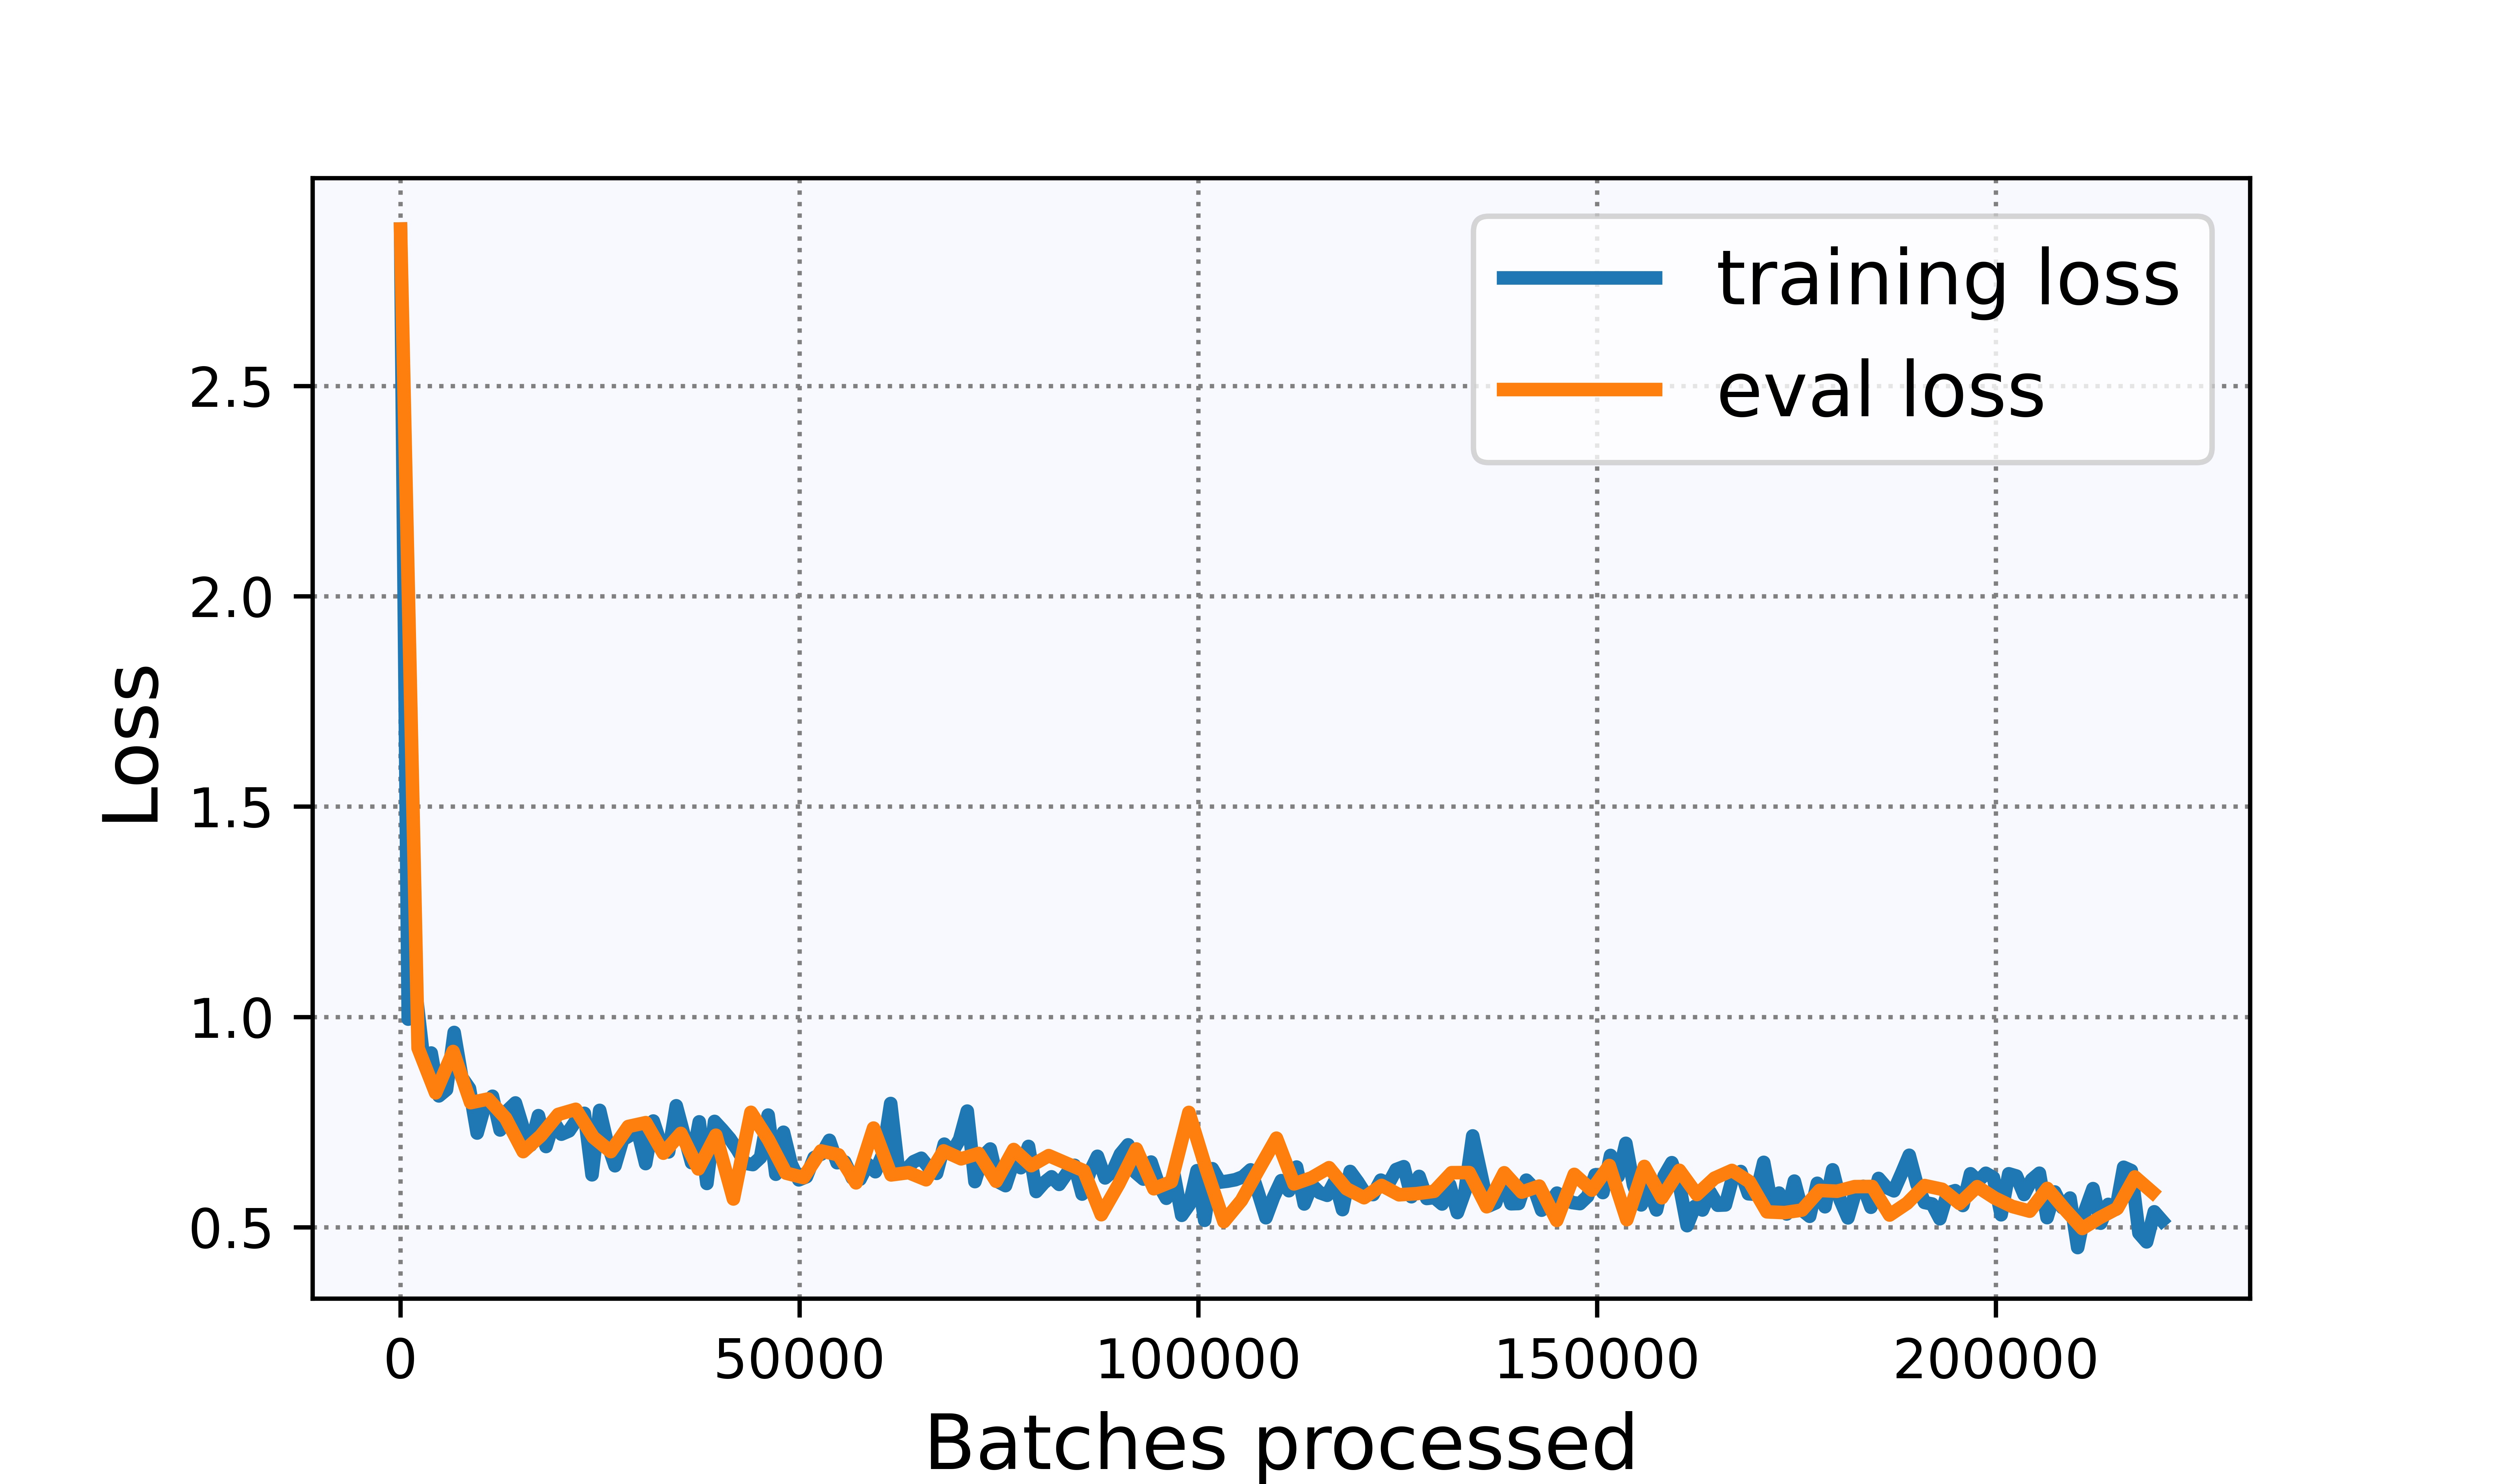
\includegraphics[width=\textwidth]{Chapters/figures/experiments/cityscapes/loss_city_seg.jpg}
        \caption{U-Net}
    \end{subfigure}
    \begin{subfigure}[b]{0.49\textwidth}
        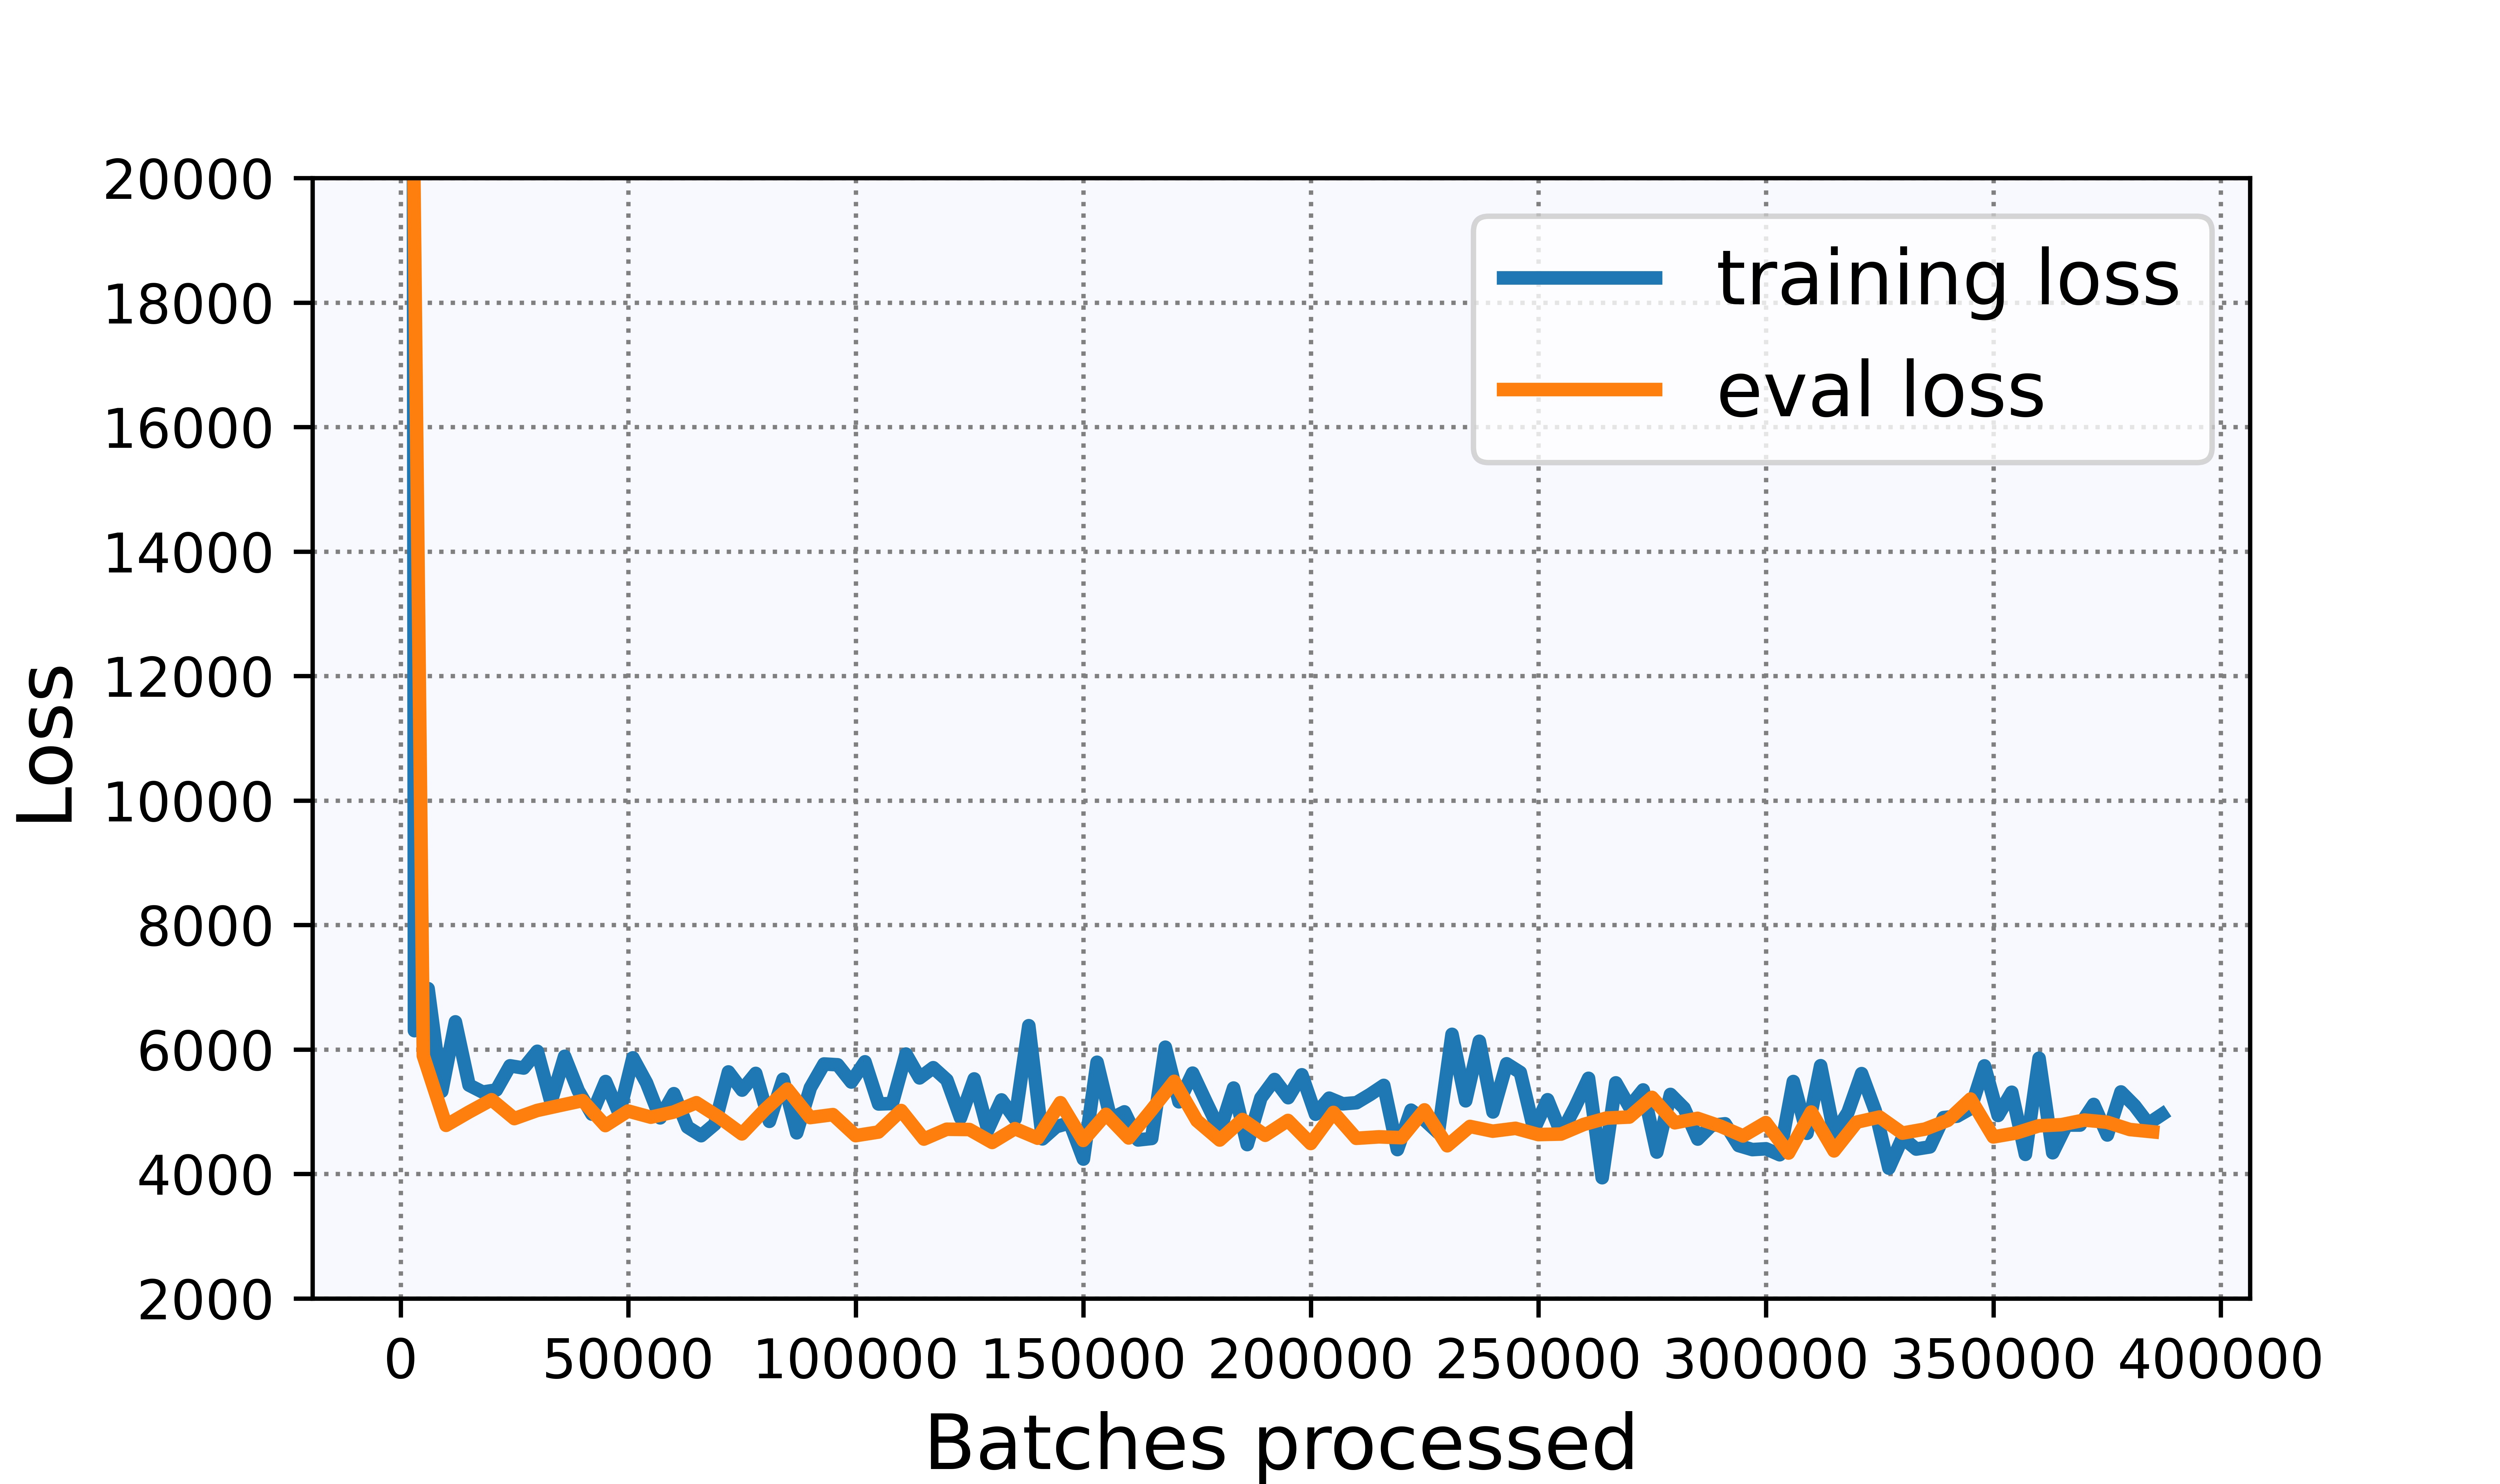
\includegraphics[width=\textwidth]{Chapters/figures/experiments/cityscapes/loss_city_ncsn.jpg}
        \caption{NSCN++}
    \end{subfigure}
    \caption[Losses of U-Net/NCSN++ on Cityscapes dataset]{Training and evaluation loss of U-Net and NCSN++ trained on the Cityscapes dataset}
\end{figure}
%
\begin{figure}[] \label{fig:3.2}
    \centering
    \begin{subfigure}[b]{0.49\textwidth}
        \centering
         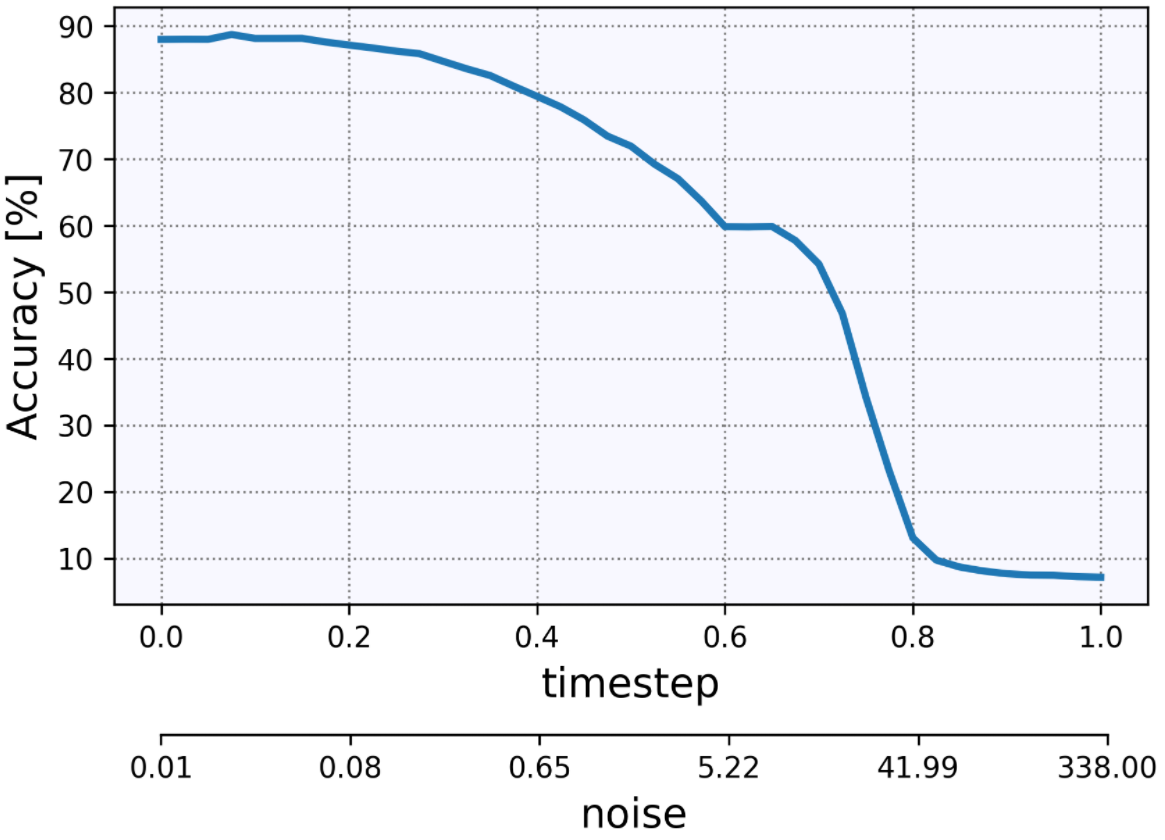
\includegraphics[width=\textwidth]{Chapters/figures/experiments/cityscapes/accuracy_cityscapes.PNG}
         \caption{Pixel Accuracy}
    \end{subfigure}
    \begin{subfigure}[b]{0.49\textwidth}
        \centering
         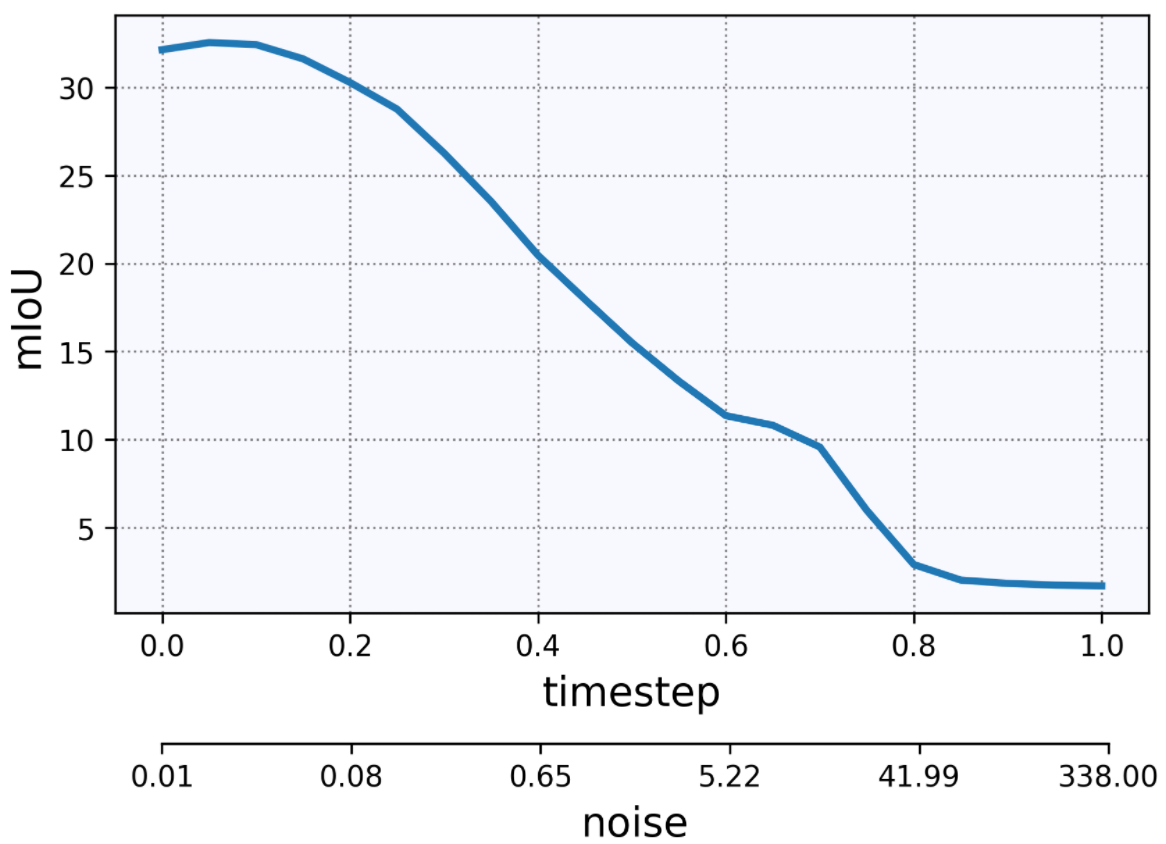
\includegraphics[width=\textwidth]{Chapters/figures/experiments/cityscapes/mIoU_cityscapes.PNG}
         \caption{Mean IoU}
    \end{subfigure}
    \caption[Pixel accuracy and mIoU for U-Net on Cityscapes dataset]{Pixel accuracy and mean IoU for noise-conditional U-Net trained on the Cityscapes dataset}
\end{figure}
%
Given the same maximum noise scale $\sigma_{max}\approx338$ as for NSCN++ and a learning rate of $0.0002$ for the Adam optimizer \cite{adam} we use for optimization, we trained the network for $600$ epochs with a batch size of $8$. In \hyperref[fig:]{Fig.\,TODO} the loss curve is shown and as with NCSN++ there is no sign of overfitting. In order to get a quantitative impression of the performance of the segmentation network we evaluated the pixel accuracy and the mean IoU separately for $41$ timesteps in $[0 ,0.8]$. The resulting curves in \hyperref[fig:]{Fig.\,TODO} show, as expected, a decrease of pixel accuracy and mIoU towards higher noise scales. It can also be seen that the values for $t=0.8$ are not significantly higher than for $t>0.8$, where the network was not trained. This indeed shows that for $t>=0.8$ the network is just guessing. A surprising finding in the two curves is the plateau region $\approx0.6<t<0.7$ for which we do not have a satisfying explanation.
%
\begin{figure} \label{fig:5.5}
    \tiny
    \centering
    \setlength\tabcolsep{-2pt}
    \begin{tabular}{ccc}
        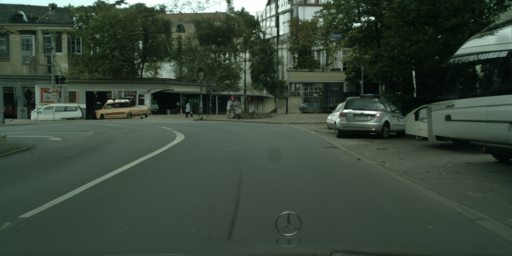
\includegraphics[width=0.33\textwidth]{Chapters/figures/experiments/cityscapes/1_uncond_sample.png} & 
        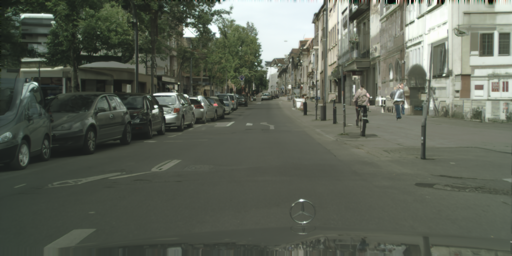
\includegraphics[width=0.33\textwidth]{Chapters/figures/experiments/cityscapes/3_uncond_sample.png} & 
        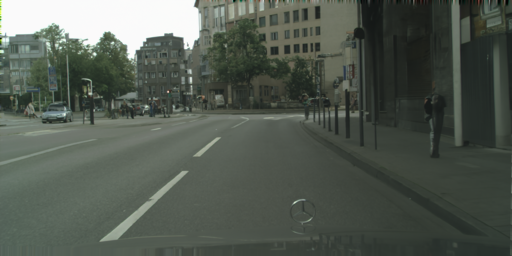
\includegraphics[width=0.33\textwidth]{Chapters/figures/experiments/cityscapes/8_uncond_sample.png}\\
        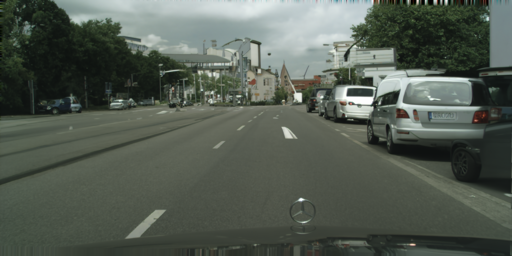
\includegraphics[width=0.33\textwidth]{Chapters/figures/experiments/cityscapes/6_uncond_sample.png} & 
        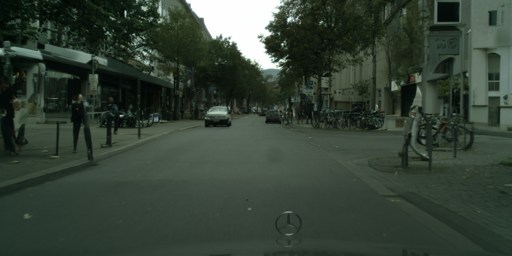
\includegraphics[width=0.33\textwidth]{Chapters/figures/experiments/cityscapes/10_uncond_sample.png} & 
        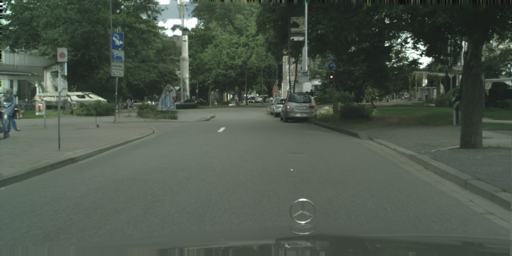
\includegraphics[width=0.33\textwidth]{Chapters/figures/experiments/cityscapes/18_uncond_sample.png} \\
    \end{tabular}
    \caption{Unconditional samples of NCSN++ trained on the Cityscapes dataset}
\end{figure}
%

\subsection{Finding optimal sampling parameters} \label{sec:5.4.4}

There are two parameters which are essential for high quality samples. The signal to noise ratio $snr$ of the Langevin sampler and the maximum scale factor $s_0$ from \hyperref[equ:5.5]{Equ.\,5.5}. 

According to \cite{score_1} a high $snr$ produces samples of higher image quality while a lower $snr$ produces samples of higher diversity. Moreover, the authors of \cite{score_1} recommend choices of $snr\in[0.05,0.2]$. We qualitatively tested values in this range on unconditional samples of the Cityscapes dataset. It is really hard to see any differences in the samples but we think that the higher sample quality manifests itself in sharper edges which in our opinion does look worse for higher values of $snr$ for the Cityscapes dataset. We therefore decide to go with a value of $snr=0.1$, but the reader is invited to form his or her own opinion by looking at the samples in \hyperref[fig:]{Fig.\,TODO}. The influence of $snr$ was also investigated on conditional samples but we were not able to find any differences in sampling quality at all.
%
\begin{figure} \label{fig:5.5}
    \tiny
    \centering
    \setlength\tabcolsep{1pt}
    \begin{tabular}{ccccc}
        $snr=0.075$ & $snr=0.1$ & $snr=0.125$ & $snr=0.15$ & $snr=0.175$ \\
        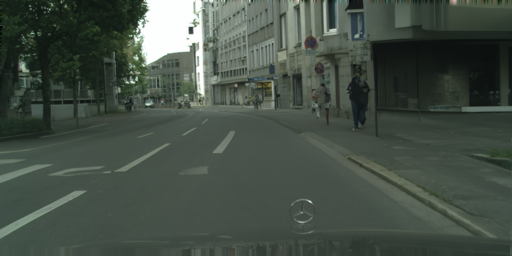
\includegraphics[width=0.19\textwidth]{Chapters/figures/experiments/cityscapes/snr/0.075/10_uncond_sample.png} & 
        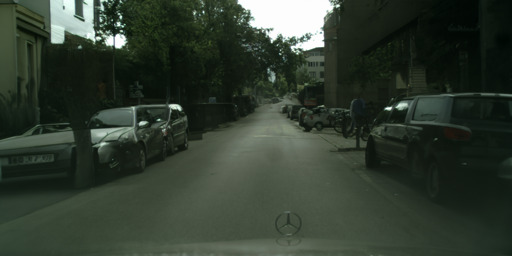
\includegraphics[width=0.19\textwidth]{Chapters/figures/experiments/cityscapes/snr/0.1/15_uncond_sample.png} &
        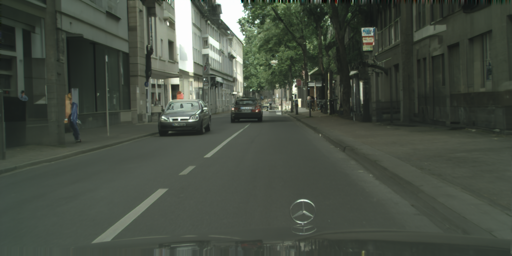
\includegraphics[width=0.19\textwidth]{Chapters/figures/experiments/cityscapes/snr/0.125/15_uncond_sample.png}& \includegraphics[width=0.19\textwidth]{Chapters/figures/experiments/cityscapes/snr/0.15/0_uncond_sample.png} & 
        \includegraphics[width=0.19\textwidth]{Chapters/figures/experiments/cityscapes/snr/0.175/0_uncond_sample.png}
        
        \\
        \includegraphics[width=0.19\textwidth]{Chapters/figures/experiments/cityscapes/snr/0.075/11_uncond_sample.png} & 
        \includegraphics[width=0.19\textwidth]{Chapters/figures/experiments/cityscapes/snr/0.1/18_uncond_sample.png} & 
        \includegraphics[width=0.19\textwidth]{Chapters/figures/experiments/cityscapes/snr/0.125/16_uncond_sample.png} & \includegraphics[width=0.19\textwidth]{Chapters/figures/experiments/cityscapes/snr/0.15/14_uncond_sample.png} &\includegraphics[width=0.19\textwidth]{Chapters/figures/experiments/cityscapes/snr/0.175/11_uncond_sample.png}
        
        \\
        \includegraphics[width=0.19\textwidth]{Chapters/figures/experiments/cityscapes/snr/0.075/4_uncond_sample.png} & 
        \includegraphics[width=0.19\textwidth]{Chapters/figures/experiments/cityscapes/snr/0.1/9_uncond_sample.png} & 
        \includegraphics[width=0.19\textwidth]{Chapters/figures/experiments/cityscapes/snr/0.125/4_uncond_sample.png} &
        \includegraphics[width=0.19\textwidth]{Chapters/figures/experiments/cityscapes/snr/0.15/17_uncond_sample.png} & \includegraphics[width=0.19\textwidth]{Chapters/figures/experiments/cityscapes/snr/0.175/8_uncond_sample.png}
    \end{tabular}
    \caption{Unconditional samples of NCSN++ for different values of $snr$}
\end{figure}
%

As seen in \hyperref[sec:5.2.5]{Sec.\,5.2.5} the maximum scale factor $s_0$ is weighting the relation between the gradients of the score network and the gradients of the semantic segmentation networks. In qualitative experiments we found that values of $s_0$ in the range $[0.0005,0.0035]$ produce visually appealing results that also comply to the given semantic map. We noticed that for higher values the samples looked slightly worse, i.e. over-saturated, and for lower values the compliance with the semantic map decreases. To quantify these effects we sampled $100$ images for $s_0=0.0005, 0.001, \dots, 0.0035$ using the same $100$ segmentation maps for each value of $s_0$. The results in \hyperref[tab:5.3]{Tab.\,5.3} confirm that the images quality (FID) decreases and the pixel accuracy as well as the mean IoU increases with higher $s_0$. We think that $s_0=0.002$ is a good compromise between image quality and semantic segmentation map compliance and therefore use this value for sampling.

\begin{table}[] \label{tab:5.3}
    \centering
    \begin{tabular}{cccccccc}
         \toprule
        $s_0$ & 0.0005 & 0.001 & 0.0015 & 0.002 & 0.0025 & 0.003 & 0.0035  \\
         \midrule
        FID & 98.78 & 100.32 & 100.59 & 102.48 & 104.52 & 104.59 & 106.40\\
        Mean IoU & 0.2422 & 0.2668 & 0.2879 & 0.3076 & 0.3023 & 0.3192 & 0.3263\\
        Pixel acc & 70.46\% & 72.33\% & 73.78\% & 74.45\% & 75.13\% & 75.33\% & 75.30\%\\
        \bottomrule
    \end{tabular}
    \caption[Evaluation of maximum scale factor on various scores]{Evaluation of maximum scale factor $s_0$ on various scores for the Cityscapes dataset}
    \label{tab:my_label}
\end{table}
\subsection{Results and Quantitative Comparisons} \label{sec:5.4.4}

With the trained models and the sampling parameters $snr=0.1$ and $s_0=0.002$ we sampled images on all $500$ testing semantic label maps of the Cityscapes dataset. We further did the same for the models CRN \cite{crn}, pix2pixHD \cite{pix2pixHD} and SPADE \cite{spade}, either using pretrained models (CRN) or training them ourselves if no pretrained models were provided (pix2pixHD, SPADE) for resolution $512\times256$. It is worth noting that these $3$ models (and adaptations of them) are state-of-the-art models, occupying $6$ of the top $10$ places in semantic image synthesis benchmarks (sorting by mIoU) on the Cityscapes dataset (see \url{https://paperswithcode.com/sota/image-to-image-translation-on-cityscapes}). 
%
\begin{figure} \label{fig:5.5}
    \small
    \centering
    \setlength\tabcolsep{1pt}
    \begin{tabular}{cccc}
        \rotatebox{90}{\text{ }Semantic Map} &
        \includegraphics[width=0.31\textwidth]{Chapters/figures/experiments/cityscapes/cond/munster_000008_000019_leftImg8bit_mask.png} & 
        \includegraphics[width=0.31\textwidth]{Chapters/figures/experiments/cityscapes/cond/munster_000139_000019_leftImg8bit_mask.png}& 
        \includegraphics[width=0.31\textwidth]{Chapters/figures/experiments/cityscapes/cond/frankfurt_000000_001236_leftImg8bit_mask.png}
        \\
        \rotatebox{90}{NCSN++ \cite{score_3}} &
        \includegraphics[width=0.31\textwidth]{Chapters/figures/experiments/cityscapes/cond/munster_000008_000019_leftImg8bit_sample.png} & 
        \includegraphics[width=0.31\textwidth]{Chapters/figures/experiments/cityscapes/cond/munster_000139_000019_leftImg8bit_sample.png} & 
        \includegraphics[width=0.31\textwidth]{Chapters/figures/experiments/cityscapes/cond/frankfurt_000000_001236_leftImg8bit_sample.png}
        \\
        \rotatebox{90}{\text{ }\text{ }\text{ }\text{ }CRN \cite{crn}} &
        \includegraphics[width=0.31\textwidth]{Chapters/figures/experiments/cityscapes/cond/munster_000008_000019_gtFine_color.png} & 
        \includegraphics[width=0.31\textwidth]{Chapters/figures/experiments/cityscapes/cond/munster_000139_000019_gtFine_color.png} & 
        \includegraphics[width=0.31\textwidth]{Chapters/figures/experiments/cityscapes/cond/frankfurt_000000_001236_gtFine_color.png} 
        \\
        \rotatebox{90}{pix2pixHD \cite{pix2pixHD}} &
        \includegraphics[width=0.31\textwidth]{Chapters/figures/experiments/cityscapes/cond/munster_000008_000019_gtFine_labelIds_synthesized_image.jpg} & 
        \includegraphics[width=0.31\textwidth]{Chapters/figures/experiments/cityscapes/cond/munster_000139_000019_gtFine_labelIds_synthesized_image.jpg} & 
        \includegraphics[width=0.31\textwidth]{Chapters/figures/experiments/cityscapes/cond/frankfurt_000000_001236_gtFine_labelIds_synthesized_image.jpg}
        \\
        \rotatebox{90}{\text{ }\text{ }SPADE \cite{spade}} &
        \includegraphics[width=0.31\textwidth]{Chapters/figures/experiments/cityscapes/cond/munster_000008_000019_leftImg8bit.png} & 
        \includegraphics[width=0.31\textwidth]{Chapters/figures/experiments/cityscapes/cond/munster_000139_000019_leftImg8bit.png} & 
        \includegraphics[width=0.31\textwidth]{Chapters/figures/experiments/cityscapes/cond/frankfurt_000000_001236_leftImg8bit.png}
    \end{tabular}
    \caption[Visual comparison of semantic image synthesis results on the Cityscapes dataset]{Visual comparison of semantic image synthesis results on the Cityscapes dataset}
\end{figure}
%

To compare our results to the ones of CRN, pix2pixHD and SPADE we use several metrics: Qualitative visual comparisons, image quality comparisons using the FID score (\hyperref[sec:fid]{Sec.\,5.4.2}) and semantic segmentation comparisons using pixel accuracy (\hyperref[sec:acc]{Sec.\,5.4.2}) and mean IoU (\hyperref[sec:fid]{Sec.\,5.4.2}). To calculate the FID scores, a python package called \textit{pytorch-fid} \cite{fid_pytorch} was used. To produce the semantic maps from the sampled images to calculate pixel accuracy and mean IoU, a pretrained version of the semantic segmentation network \textit{Dilated Residual Network} (DRN) \cite{drn} was used. The reason for this choice is that DRN generally performs very well on the Cityscapes dataset, that DRN was used in similar model comparisons in \cite{pix2pix} and \cite{spade} and that we want to prevent bias by using another network than U-Net for our analysis.
 
The visual comparison of some explicitly selected samples is presented in \hyperref[fig:]{Fig.\,TODO}. In our opinion our results have the possibility to outperform the visual appearance of the other models. However, there are two very important restrictions to this opinion: First, our samples do not always look better, therefore we provide more, uncurated samples in the appendix TODO. And second, apparently our model is very bad at sampling fine structures of the semantic map, e.g. persons or street signs. 

This poor performance on fine structure can also be seen in the pixel accuracy and mIoU scores in \hyperref[tab:5.4]{Tab.\,5.4}. While the pixel accuracy score is acceptable in comparison to the other models, the mIoU is not. For the quality comparison using FID scores in \hyperref[tab:5.5]{Tab.\,5.5} we conclude that our model perform quite good in comparison to the other models.

All in all we conclude to things for this experiment: First, our approach of semantic images synthesis using SGMs is capable to keep up with state-of the-art models. Second, there is room for improvements especially in semantic map compliance for fine structures. We think that a more complex noise-conditioned semantic segmentation network than the relatively simple U-Net could increase mean IoU and pixel accuracy scores if being better for higher noise scales. We also think that such a network would increase sample quality as we suppose that the main factor for bad quality is not NCSN++ but the semantic segmentation network performing poor on high noise scales.

\begin{table}[] \label{tab:5.4}
    \centering
    \begin{tabular}{ccccc|c}
         \toprule
         &  CRN \cite{crn} & pix2pixHD \cite{pix2pixHD} & SPADE \cite{spade} & NCSN++ \cite{score_3} & Oracle\\
         \midrule
        Mean IoU & 0.5345 & 0.5172 & \textbf{0.6191} & 0.3089 & 0.6181\\
        Pixel acc & 74.86\% & 79.59\% & \textbf{81.50}\% & 74.95\% & 81.00\%\\
        \bottomrule
    \end{tabular}
    \caption[Semantic segmentation scores on Cityscapes dataset]{Semantic segmentation scores on results by different
methods on the Cityscapes dataset. Oracle describes scores on original images}
    \label{tab:my_label}
\end{table}

\begin{table}[] \label{tab:5.5}
    \centering
    \begin{tabular}{ccccc}
        \toprule
         &  CRN \cite{crn} & pix2pixHD \cite{pix2pixHD} & SPADE \cite{spade} & NCSN++ \cite{score_3}\\
         \midrule
         FID & 71.43 & 83.91 & \textbf{56.03} & 66.46\\
         \bottomrule
    \end{tabular}
    \caption[FID scores on results by different methods on the Cityscapes dataset]{FID scores on results by different methods on the Cityscapes dataset}
    \label{tab:my_label}
\end{table}



\section[Synthesizing high resolution landscapes]{Synthesizing high resolution landscapes%
    \sectionmark{Flickr landscapes}} \label{sec:5.5}
\sectionmark{Flickr landscapes}
In the experiment on the Cityscapes dataset in \hyperref[sec:5.4]{Sec.\,5.4} we found that our semantic image synthesis model performs poor on fine structures like persons and traffic lights but good on coarse structures like streets, cars and vegetation. For that reason we want to test our model on a dataset with less labels and more coarse structures. Inspired by impressive results from Esser and Rombach \cite{taming} on a dataset called \textit{S-FLCKR} which contains $79266$ landscape images from the image platform Flickr, we chose to test our model on this dataset. The semantic maps for these images were generated with a COCO-stuff \cite{coco_stuff} segmentation network which also contains some landscape labels. Since these generated semantic maps are far from perfect, they do not represent \textit{ground truth} and therefore most quantitative measures cannot be applied to our results.

\subsection{Training and Sampling}
For training of our models we use the same model parameters as described in \hyperref[sec:5.4]{Sec.\,5.4}, except for the maximum Euclidean distance, which was calculated to be $\sigma_{max}\approx440$. With a batch size of $8$ resp. $22$, NCSN++ and U-Net were trained for $30$ resp. $10$ epochs. One important deviation from the training procedure for the Cityscapes dataset is that the landscape images are of various resolutions up to $1024\times2048$ and so the models were trained on $512\times512$ randomly cropped and horizontally flipped images. This higher training resolution will allow us to sample images of higher resolution but also drastically increases vRAM usage during NSCN++ training to $\approx80GB$ and sampling time to $\approx1h$ per sample. We present loss curves as well as mIoU and pixel accuracy curves in \hyperref[fig:]{Fig.\,TODO} and \hyperref[fig:]{Fig.\,TODO}.

In order to get a semantic segmentation network that works well on landscapes, we condensed the $182$ class labels of COCO-stuff to $6$ landscape classes – Sea, Mountain, Grass, Forest, Sky, Clouds – and one "unlabeled" class. During training the model is penalized only for incorrect predictions on the $6$ landscape images. For sampling we drew our own semantic maps using the $6$ classes described above.

For the sampling parameters $s_0$ and $snr$, no quantitative experiments were conducted, because the enormous sampling time of $\approx1h$ per image did not allow us to accumulate enough samples for an extended analysis. Qualitative examinations together with the insights from \hyperref[sec:5.4.4]{Sec.\,5.4.4} let us conclude that $s_0=0.1$ and $snr=TODO$ work fine for the S-FLCKR dataset. A few unconditional sample can be found in \hyperref[fig:]{Fig.\,TODO}.
%
\subsection{Results}

\section[ADE20K - Pushing the model to its limits]{ADE20K - Pushing the model to its limits%
    \sectionmark{ADE20K}} \label{sec:5.6}
\sectionmark{ADE20K}
In this experiment we want to qualitatively evaluate the performance of the proposed semantic image synthesis model on the ADE20K dataset \cite{ade20k}. The goal is to get a feeling for the limits of the current model, especially for the relatively simple U-Net semantic segmentation network. The ADE20K dataset is generally difficult to learn due to its large variety of scenes and the sample quality is to be expected poorer than for simple datasets such as Cityscapes. 
\subsection{The ADE20K dataset}
The ADE20K dataset \cite{ade20k}  is designed for semantic segmentation and semantic image synthesis of images with no general type of scene. It consists of $25574$ training and $2000$ testing images of various resolutions which all come with a fine annotated label map. The images span $365$ different scenes and contain $707{,}868$ unique objects from $3{,}688$ categories. The $365$ scenes are very diverse, containing scenes of urban buildings, landscapes, rooms, such as bathrooms and kitchens, scenes of daily life and many more. 
\subsection{Training and Sampling}
As in the previous experiments we did not change any complex model parameters. The maximum Euclidean distance between the images was calculated to $\sigma_{max}\approx394$. We then trained both the NSCN++ and the U-Net on $256\times256$ pixel randomly cropped images and chose a batch size of $16$ for the NCSN++ and $64$ for U-Net. NCSN++ and U-Net were trained for $220$ resp. $150$ epochs.

Sampling parameters were only qualitatively investigated and it was found that a value of $snr=0.075$ for the signal-to-noise-ratio and $s_0=0.0025$ for the maximum scale factor produces decent results. As we will see in \hyperref[sec:5.6.3]{Sec.\,5.6.3}, there is no need for parameter fine-tuning since the resulting samples defy any quantitative analysis.

The loss curves of U-Net and NCSN++ are presented in \hyperref[fig:]{Fig.\,TODO}. We also show some unconditioned samples in \hyperref[fig:]{Fig.\,TODO} which convincingly show why the ADE20K is considered a dataset for semantic image synthesis and not for general image generation.

%
\begin{figure}[] \label{fig:3.2}
    \centering
    \begin{subfigure}[b]{0.49\textwidth}
        \includegraphics[width=\textwidth]{Chapters/figures/experiments/ade/loss_ade_seg.jpg}
        \caption{U-Net}
    \end{subfigure}
    \begin{subfigure}[b]{0.49\textwidth}
        \includegraphics[width=\textwidth]{Chapters/figures/experiments/ade/loss_ade_ncsn.jpg}
        \caption{NSCN++}
    \end{subfigure}
    \caption[Losses of U-Net/NCSN++ on ADE20K dataset]{Training and evaluation loss of U-Net and NCSN++ trained on the ADE20K dataset}
\end{figure}
%
\begin{figure}[]
    \centering
    \begin{subfigure}[b]{0.49\textwidth}
        \centering
         \includegraphics[width=\textwidth]{Chapters/figures/experiments/ade/accuracy_ade20k.PNG}
         \caption{Pixel Accuracy}
    \end{subfigure}
    \begin{subfigure}[b]{0.49\textwidth}
        \centering
         \includegraphics[width=\textwidth]{Chapters/figures/experiments/ade/mIoU_ade20k.PNG}
         \caption{Mean IoU}
    \end{subfigure}
    \caption[Pixel accuracy and mIoU for U-Net on ADE20K dataset]{Pixel accuracy and mean IoU for noise-conditional U-Net trained on the ADE20K dataset}
\end{figure}
%
\begin{figure} 
    \tiny
    \centering
    \setlength\tabcolsep{-2pt}
    \begin{tabular}{ccccc}
        \includegraphics[width=0.20\textwidth]{Chapters/figures/experiments/ade/2_uncond_sample.png} & 
        \includegraphics[width=0.20\textwidth]{Chapters/figures/experiments/ade/3_uncond_sample.png} & 
        \includegraphics[width=0.20\textwidth]{Chapters/figures/experiments/ade/4_uncond_sample.png} & 
        \includegraphics[width=0.20\textwidth]{Chapters/figures/experiments/ade/10_uncond_sample.png} &
        \includegraphics[width=0.20\textwidth]{Chapters/figures/experiments/ade/11_uncond_sample.png}
    \end{tabular}
    \caption{Unconditional samples of NCSN++ trained on the ADE20K dataset}
\end{figure}


\subsection{Results} \label{sec:5.6.3}

Some final samples of semantic image synthesis on the ADE20K dataset are presented in \hyperref[fig:]{Fig.\,TODO}. It is quite clearly visible that the sample images have only remotely anything to do with the original images. We do not see the reasons for this in the image quality of the NCSN++. It is true that the unconditional samples are not very realistic but this was expected for a dataset such as ADE20K. Conversely, we even find that the unconditional samples of NCSN++ capture the character of the dataset quite well, and besides, the logical information should be provided by the semantic segmentation network anyway. Therefore, we suspect that the poor sample quality is more likely due to the semantic segmentation network not performing well on noisy images, which is supported by the findings \hyperref[fig:]{Fig.\,TODO}. However, we are not entirely sure why this poor segmentation performance leads to the very artistic-looking image style, as we see no evidence of this behavior in unconditional samples.

From the results of this experiment, we conclude that a simple noise-conditioned U-net simply does not perform well enough to be used in semantic image synthesis with SGMs for complex datasets. In order to generate good samples on such datasets, we assume that a semantic segmentation network specifically designed for noise-conditioned semantic segmentation must be developed.

\begin{figure} \label{fig:5.5}
    \tiny
    \centering
    \setlength\tabcolsep{-2pt}
    \begin{tabular}{ccccc}
        \includegraphics[width=0.20\textwidth]{Chapters/figures/experiments/ade/ADE_val_00000210_original.png} & 
        \includegraphics[width=0.20\textwidth]{Chapters/figures/experiments/ade/ADE_val_00000393_original.png} & 
        \includegraphics[width=0.20\textwidth]{Chapters/figures/experiments/ade/ADE_val_00001998_original.png} & 
        \includegraphics[width=0.20\textwidth]{Chapters/figures/experiments/ade/ADE_val_00001993_original.png} &
        \includegraphics[width=0.20\textwidth]{Chapters/figures/experiments/ade/ADE_val_00001430_original.png}\\
        \includegraphics[width=0.20\textwidth]{Chapters/figures/experiments/ade/ADE_val_00000210_sample.png} & 
        \includegraphics[width=0.20\textwidth]{Chapters/figures/experiments/ade/ADE_val_00000393_sample.png} & 
        \includegraphics[width=0.20\textwidth]{Chapters/figures/experiments/ade/ADE_val_00001998_sample.png} &
        \includegraphics[width=0.20\textwidth]{Chapters/figures/experiments/ade/ADE_val_00001993_sample.png} &
        \includegraphics[width=0.20\textwidth]{Chapters/figures/experiments/ade/ADE_val_00001430_sample.png}
        
    \end{tabular}
    \caption[Semantically synthesized images for the ADE20Kdataset]{Semantically synthesized images for the ADE20Kdataset. \\\textit{Bottom}: Synthesized Images, \textit{Top}: Corresponding real images}
\end{figure}




